%%%--- Template for bachelor thesis at SfS, based on template
%%%--- for Diploma and Master thesis------
%%%------
\documentclass[11pt,a4paper,twoside,openright]{report}
\usepackage[english]{ETHDAsfs}%--> ETHDASA + fancyhdr + ... "umlaute"
%  + sfs-hyper -> hyperref 

\usepackage{pdfpages}%%to include the confirmation of originality (plagiarism
\usepackage{amsbsy}%% for \boldsymbol and \pmb{.}
\usepackage{amssymb}%% calls  amsfonts...
\usepackage{graphicx}%-- für PostScript-Grafiken (besser als  psfig!)
%\usepackage[draft]{graphicx} % grafics shown as boxes --> faster compilation
%
\usepackage[longnamesfirst]{natbib}%was {sfsbib}%- Für  Literatur-Referenzen
%           ^^^^^^^^^^^^^^ 1) "Hampel, Ronchetti, ..,"  2) "Hampel et al"
% Engineers (and other funny people) want to see [1], [2] 
% ---> use 'numbers' : \usepackage[longnamesfirst,number]{natbib}
%
%
\usepackage{texab}%- 'tex Abkürzungen' /u/sfs/tex/tex/latex/texab.sty
        %%- z.B.  \R, \Z, \Q, \Nat für reelle, ganze, rationale, natürl. Zahlen;
        %%-       \N   (Normalvert.)  \W == Wahrscheinlichkeit .....
        %%-  \med, \var, \Cov, \....
        %%-  \abs{x} == |x|   und   \norm{y} ==  || y ||   (aber anständig)
%% NOTE: texab contains many useful definitions and "shortcuts". It is
%% worth to open the file and have a look at them. HOWEVER, some
%% definitions are a bit can lead to conflicts with other packages. You
%% might for example want to comment out the line defininf \IF as an
%% operator when working with the algorithmic package, or to comment out
%% the line defining a command \Cite with working with the Biblatex package  
\usepackage{amsmath}
%\usepackage{mathrsfs}% Raph Smith's Formal Script font --> provides \mathscr
\usepackage[utf8]{inputenc}% <<------- Unicode, *NOT* iso-latin1 !
\usepackage{ae}% A[lmost] E[uropean] Fonts
\usepackage{enumerate}% Fuer selbstdefinierte Nummerierungen
%--------
\usepackage{relsize}%-> \smaller (etc) used here
\usepackage{color} %% to allow coloring in code listings
\usepackage{Sweave}
\usepackage{listings}% Fuer R-code, C-code, ....  and settings for these:
\usepackage{m-floating}% for tables and figures.

\definecolor{Mygrey}{gray}{0.75}% for linenumbers only!
\definecolor{Cgrey}{gray}{0.4}% for comments
\lstloadlanguages{R}
%%--- first version of "listings of R"-style : ---------------------------
% %% using \smaller here: makes R code listings use a *small* font:
% \lstset{language=R,basicstyle=\smaller[2],commentstyle=\rmfamily\smaller,
%   showstringspaces=false,xleftmargin=4ex,
%   literate={<-}{{$\leftarrow$}}1 {~}{{$\sim$}}1}
% \lstset{escapeinside={(*}{*)}} % for (*\ref{ }*) inside lstlistings (Scode) 
%\newcommand{\lil}[1]{\lstinline|#1|}
%%--- newer version of "listings of R"-style : ---------------------------
\lstset{%% Help, e.g. --> https://en.wikibooks.org/wiki/LaTeX/Source_Code_Listings
language=R,
basicstyle=\ttfamily\scriptsize,%%- \small > \footnotesize > \scriptsize > \tiny
%commentstyle=\ttfamily\color{Cgrey},
commentstyle=\itshape\color{Cgrey},
numbers=left,
numberstyle=\ttfamily\color{Mygrey}\tiny,
stepnumber=1,
numbersep=5pt,
backgroundcolor=\color{white},
showspaces=false,
showstringspaces=false,
showtabs=false,
frame=single,
tabsize=2,
captionpos=b,
breaklines=true,
%breakatwhitespace=false,
keywordstyle={},
morekeywords={},
xleftmargin=4ex, 
literate={<-}{{$\leftarrow$}}1 {~}{{$\sim$}}1}
\lstset{escapeinside={(*}{*)}} % for (*\ref{ }*) inside lstlistings (Scode) 
%%----------------------------------------------------------------------------

%%------- Theoreme ---
\newtheorem{definition}{Definition}[subsection]
\newtheorem{lemma}[definition]{Lemma}
\newtheorem{theorem}[definition]{Theorem}
\newtheorem{Coro}[definition]{Corollary}
\theoremstyle{definition} 
\newtheorem{example}[definition]{Example}
\newtheorem*{note}{Note}
\newtheorem*{remark}{Remark}

\DeclareMathOperator*{\plim}{plim}
\def\MR#1{\href{http://www.ams.org/mathscinet-getitem?mr=#1}{MR#1}}

\newcommand{\Lecture}[3]{\marginpar{#3.#2.#1}}
\newcommand{\Fu}{\mathcal{F}}
\newcommand{\aatop}[2]{\genfrac{}{}{0pt}{}{#1}{#2}}

%\renewcommand{\theequation}{\arabic{equation}}
\numberwithin{equation}{subsection}
%\includeonly{}

%\pscompress %--compress the Epsf .ps files and produce .bb -- WHEN dvips is run
%\psdraft%--- for quick pre-viewing (only shows frames)

%%%%%%%%%%%%%%%%%%%%%%%%%%%%%%%%%%%%%%%%%%%%%%%%%
%%% Path for your figures                      %%%
%%%%%%%%%%%%%%%%%%%%%%%%%%%%%%%%%%%%%%%%%%%%%%%%%
% Set the paths where all figures are taken from:
% \graphicspath{{/u/mueller/MA/Figures1/}{/u/mueller/MA/Figures2/}}

%%%%%%%%%%%%%%%%%%%%%%%%%%%%%%%%%%%%%%%%%%%%%%%%%
%%% Define your own commands here             %%%
%%%%%%%%%%%%%%%%%%%%%%%%%%%%%%%%%%%%%%%%%%%%%%%%%
\newcommand{\Bruch}[2]{{}^{#1}\!\!/\!_{#2}}
\renewcommand{\labelenumi}{\roman{enumi}.)}


\newenvironment{Rgraph}[1][0.6]{\vspace{-5mm}%
%% NOTA BENE: MM thinks we should  replace the "vspace" by using pdfCrop
\begin{center} \setkeys{Gin}{width=#1\textwidth}}{\end{center}}




\begin{document}
\bibliographystyle{chicago}% ---> Hampel,F., E.Ronchetti,... W.Stahel(1986) ...
 %was \bibliographystyle{sfsbib}\citationstyle{dcu} %OR DEFAULT : \citationstyle{agsm}

\pagenumbering{roman}%- roman numbering for first few pages

%%%%%%%%%%%%%%%%%%%%%%%%%%%%%%%%%%%%%%%%%%%%%%%%%
%%% Title page                                %%%
%%%%%%%%%%%%%%%%%%%%%%%%%%%%%%%%%%%%%%%%%%%%%%%%%
 \period{Winter 2019} %e.g. Winter 2019
 \dasatype{Bachelor Thesis}
 \students{Nicolas Trutmann} %e.g. Patrick M\"uller
 \mainreaderprefix{Advisor:}
 \mainreader{Dr. Martin M\"achler} %e.g. Prof. Dr. Martin M\"achler
 \alternatereaderprefix{}
 \alternatereader{}
 \issuedate{June 12th 2019} %e.g. September 15th 2019
 \submissiondate{November 1st 2019} %e.g. February 31st 2019
 \title{Comparing the EM-algorithm and Maximum Likelihood Estimation Using the 
        Cholesky Decomposition} %title of your work

 \maketitle%- Titelseite wird abgeschlossen
 %%~~~~~~~~~~~~~~~~~~~~~~~~~~~~~~~~~~~~~~~~

%%%%%%%%%%%%%%%%%%%%%%%%%%%%%%%%%%%%%%%%%%%%%%%%%
%%% Insert here acknowledgements and abstract %%%
%%%%%%%%%%%%%%%%%%%%%%%%%%%%%%%%%%%%%%%%%%%%%%%%%
 \newpage
\begin{abstract}
	The intent of this work is to compare The EM algorithm to an MLE approach in 
    the	case of multivariate normal mixture models. 
	The EM algorithm is widely used in statistics and is proven to converge, 
	however in pathological cases convergence slows down considerably. 

    Our proposed alternative consists of a clustering algorithm as 
    initialization step, followed by a parametrization step, that is then fed 
    into a general optimizer.

    We compare two implementations of each algorithm with two different 
    initialization strategies by judging their performance in model selection.
    Model selection is decided by the Bayesian Information Criterion (BIC).

    The results are promising. In many cases MLE is equal or better than EM.
    It is certainly a competitive model selection strategy. This could yield
    improvements in the field of model selection. The algorithm design is also 
    versatile and translates easily to other problems.
\end{abstract}

%%%%%%%%%%%%%%%%%%%%%%%%%%%%%%%%%%%%%%%%%%%%%%%%%
%%% Table of contents and list of figures and %%%   
%%% tables (no need to change this usually)   %%%
%%%%%%%%%%%%%%%%%%%%%%%%%%%%%%%%%%%%%%%%%%%%%%%%%
\newpage
\tableofcontents
\newpage
\listoffigures
\newpage
\listoftables
\cleardoublepage

\pagenumbering{arabic}%--- switch back to standard numbering 


%%%%%%%%%%%%%%%%%%%%%%%%%%%%%%%%%%%%%%%%%%%%%%%%%
%%% Your text... Either write here directly,  %%%
%%% or even better: write in separate files   %%%
%%% that you just have to include here.       %%% 
%%%%%%%%%%%%%%%%%%%%%%%%%%%%%%%%%%%%%%%%%%%%%%%%%
\chapter{Introduction to normal mixture models}



\section{Definitions}
\label{sec:def}

A good and thorough introductory book is the work of \cite{McL00} and
the reader is encouraged to study it to learn in depth about normal mixtures
and clustering. 
We will here give a short overview of normal mixtures to fix notation and 
nomenclature.
The motivating idea behind mixture models is, that in real world examples
a sample might be suspected to arise from more than one population or be 
more simply modelled by several overlaid distributions.
The example of this, that is generally considered to be the first of this kind,
is the one by Karl Pearson, who fitted two normal distributions with different 
means and variances to a dataset.
In his book, \cite{Pea96}[Section 4.d.; page 266], Pearson analyzed measurements
of forehead to body length of crabs sampled from the bay of Naples. His mixture 
model-based approach suggested, that the crabs were evolving into two new 
subspecies.
This is a historically important example, because it presents statistical 
evidence of evolution in process.

While the theory of mixture models holds for a much broader class of 
distributions, we restrict ourselves here to the case of normal mixture models,
because normal distributions allow for a parsimonious parametrization, that is 
of interest to study.

This parametrization is the $\pmb{LDL}\top$ decomposition, a variation of the 
Cholesky decomposition, which allows for a very 
simple parametrization and a straightforward connection between degrees of 
freedom and necessarily generated numerical values. This will be explained 
further in section \ref{sec:models}.

But before we delve deeper into the topic of this research, we first need to 
define the concept of a normal mixture model:

Let $ \mu \in \mathbb{R}^p , \quad \Sigma \in \mathbb{R}^{p \times p} $ be
symmetric positive definite and $ \phi(- ; \mu, \Sigma) $ be the normal 
distribution with mean $ \mu $ and covariance matrix $ \Sigma $ with density 
function:

\begin{equation} 
    \phi(\pmb{x;\mu,\Sigma})=
    \frac{\exp(-\frac{1}{2}(\pmb{x-\mu})\pmb{\Sigma}^{-\frac{1}{2}}(\pmb{x-\mu})^\top)}
         {\sqrt{(2\pi)^k \det{\pmb{\Sigma}}}}  
\end{equation}

for $\pmb{x} \in \mathbb{R}^p$.

Since we are studying mixture models, we will need several overlapping of 
normal distributions, of differing means and covariance. Therefore, we choose
notation allowing us to refer to the components in shorthand. Let us assume we
have $K \in \mathbb{N}$ normal distributions with means and covariance 
$\pmb{\mu}_k, \pmb{\Sigma}_k,\quad k \in \{1, \dots , K\}$, then we fix:

\begin{equation} 
    \phi_k(\pmb{x}) := \phi(\pmb{x;\mu_k, \Sigma_k})
    \label{eqn:phik}
\end{equation}

And going forward, we will refer to components by the subscript $k$.

\begin{definition}
    Suppose we have a random sample $ \pmb{Y}_1, \dots , \pmb{Y}_n $, where
    $\pmb{Y}_i$ is a $p$-dimensional random vector with probability density 
    function $ \pmb{Y}_i \sim f(\pmb{y}_i) $ on $\mathbb{R}^p$.

    We assume that the density $ f(\pmb{y}_i) $ of $ \pmb{Y}_i $ can 
    be written in the form: 
    \begin{equation} 
        f(\pmb{y}_i) = \sum_{k=1}^{K} \pi_k \phi_k (\pmb{y}_i)
        \label{eqn:mixture}
    \end{equation}
    The $\phi_k$ are normal distributions and are called the mixture components
    with parameters $\pmb{\mu}_k$ and $\pmb{\Sigma}_k$ as described above 
    (\ref{eqn:phik}).
    The $ \pi_k $ are called the component densities of the mixture and are
    constrained by the rules $\pi_k > 0$ and $\sum_k \pi_k = 1$.
\end{definition}

For 'large' datasets there are applicable constraints to the $\pmb{\Sigma}_k$, 
that reduce the number of necessary parameters. These, for example, assume that 
all components have the same covariance, or have certain restrictions placed on 
them. We will give a detailed description of the models assumed in this thesis 
in section \ref{sec:models}.


\section{The EM-algorithm in Sketch}
\label{sec:sketch}

With this definition, we immediately face the problem of how to fit these
mixture components to given data. A popular algorithm to solve this problem 
is the {\bf E}xpectation-{\bf M}aximization algorithm, abbreviated as 
EM-algorithm.

We give here a sketch of the EM-algorithm in the case of normal mixtures. This 
roughly follows the content in \cite{McL00}. For a more thorough treatment of 
the matter see chapter 3.

Suppose we have a $p-$dimensional dataset of $n$ samples $\pmb{y}_1, \dots ,\pmb{y}_n$,
onto which we would like to fit a $K$ component normal mixture with mixture
components $\phi_k,\ k \in {1,\dots , n}$. 

For the EM-algorithm further parameters are introduced. These are denoted
$\tau_j(\pmb{y}_i)$ and they represent the posterior probabilities that 
observation $i$ is a member of component $j$.

The EM-algorithm is a two step, iterative process consisting of an 'e'-step
and an 'm'-step.
In the e-step the expectation of component membership is updated.

\begin{equation} 
    \tau_j(\pmb{y}_i;\Psi) = \phi_j(\pmb{y}_i)/ \sum_{k=1}^K \phi_k(\pmb{y}_i)
\end{equation}

and in the m-step given the component membership information we update the 
component means and covariances by weighted versions of the usual estimators.
\begin{equation}
    \pmb{\mu}_j = \sum_{i=1}^n \tau_j(\pmb{y}_i)\pmb{y}_i / \sum_{j=1}^n \tau_j(\pmb{y}_i)
\end{equation}
\begin{equation}
    \pmb{\Sigma}_j = \sum_{i=1}^n \tau_j(\pmb{y}_i) (\pmb{y}_i- \pmb{\mu}_j)(\pmb{y}_i-\pmb{\mu}_j)^\top /  \sum_{i=1}^n \tau_j(\pmb{y}_i)
\end{equation}

There remains to be stated how to start the algorithm. Since both steps of the
algorithm depend on data from the other, the EM-algorithm needs some form of 
initialization step.
Most popular implementations use some form of pre clustering and use the 
EM-algorithm as subsequent tools to fit the data. The R-package {\tt mclust} 
for example uses hierarchical agglomerative clustering \cite{Scr16}.


\section{Choice of Notation}
\label{sec:notation}

The classification of models in this paper relies heavily on the work of 
\cite{Cel95}, however, out of necessity for clarity, we break with their 
notation. So as to not confuse the reader we describe here in depth the 
differences between \cite{Cel95} and this work.

The basis of classification in \cite{Cel95} is the decomposition of a
symmetric matrix into an orthogonal and a diagonal component.
A symmetric positive definite matrix $\Sigma$ can be decomposed as

\begin{equation} 
    \Sigma = \lambda \pmb{D} \pmb{A} \pmb{D}^{\top}
\end{equation}

with $\pmb{D}$ an orthogonal matrix and $\pmb{A}$ a diagonal matrix and
$\lambda = \sqrt[\uproot{3}p]{det(\Sigma)}$ the $p$-th root of the determinant 
of $ \Sigma $.

This decomposition has an appealing geometric interpretation, with $ \pmb{D} $ 
as the \textit{orientation} of the distribution, $ \pmb{A} $ the \textit{shape},
and $ \lambda $ the \textit{volume}. The problem of notation comes from standard 
conventions in linear algebra, where the letters $A$ and $D$ are usually 
occupied by arbitrary and diagonal matrices respectively. Furthermore, we intend
to apply a variant of the Cholesky decomposition to $ \Sigma $, the 
$ \alpha\pmb{L}\pmb{D}\pmb{L}^{\top} $ decomposition. This obviously raises some
conflicts in notation.

Therefore we, from here on, when referring to the decomposition as described by 
\cite{Cel95}, will use the following modification of notation:

\begin{gather} 
    \pmb{D} \longmapsto \pmb{Q} \\
    \pmb{A} \longmapsto \pmb{\Lambda} \\
    \lambda \longmapsto \alpha  \\
    \Sigma = \lambda \pmb{D} \pmb{A} \pmb{D}^\top \longmapsto
        \alpha \pmb{Q} \pmb{\Lambda} \pmb{Q}^\top
\end{gather}

These were chosen according to general conventions of linear algebra. $ \pmb{Q} $
is usually chosen for orthonormal matrices; $ \pmb{\Lambda} $ is often a choice 
for diagonal matrices of eigenvectors and $ \alpha $ was chosen arbitrarily.


\section{Models of Covariance Matrices}
\label{sec:models}

As mentioned in the introduction, there are ways to constrain the covariance 
matrices. There are instances where the resulting loss of information is seen 
as acceptable, for example if, through consideration of the data, that a 
simplified model is acceptable. Another is if the sheer size of the data makes 
application of full generality impossible.

With the above mentioned decomposition, we have the following options to 
constrain the covariance model:

\begin{itemize}
    \item We restrict the complexity of the decomposition, substituting it with 
        a simpler component.
    \item We restrict the variability of the mixture components, fixing a part 
        of the decomposition to be equal.
\end{itemize}

Let us look at the first case. We take the decomposition of a covariance matrix
as $\Sigma = \alpha \pmb{Q\Lambda Q}^\top$. Of these, we can simplify the 
structure of $\pmb{Q}$ and $\pmb{\Lambda}$, by replacing them with the identity.
If we set $\pmb{Q}=\mathrm{Id}$, we lose the freedom of orientation and if we 
set $\pmb{\Lambda}=\mathrm{Id}$ we restrict ourselves to spherical 
distributions. Of course, we cannot restrict $\pmb{\lambda}$ while letting 
$\pmb{q}$ free, since

\begin{equation} 
    \pmb{Q\Lambda Q}^\top = \pmb{Q}\mathrm{Id}\pmb{Q}^\top = \mathrm{Id}
\end{equation}

The second restriction simply means we hold the decomposition fixed throughout 
all covariance matrices.

There is however an issue with the Cholesky decomposition. For ten out of 
fourteen cases defined by \cite{Cel95}, there exists a canonical translation of
decompositions, but for four of them no translation is possible.

The six diagonal cases need no translation; the eigen- and Cholesky 
decomposition are equal to the non decomposed form. For the non diagonal cases 
note that for a given symmetric positive definite matrix $\Sigma$ we have 
decompositions:

\begin{equation}
    \Sigma = \alpha \pmb{Q \Lambda Q}^\top \quad \Sigma =\alpha \pmb{L D L}^\top
\end{equation}

Since in both cases the enclosing matrices $ \pmb{Q} $ and $ \pmb{L} $ have 
determinant $1$ the determinant of $\Sigma$ falls entirely on $ \alpha $.
Therefore $ \alpha $, in these particular decompositions, is equal for both.
\cite{Cel95} vary $\sigma$ by either varying or holding fixed the volume 
$(\alpha / \alpha_k)$, shape $(\pmb{\Lambda} / \pmb{\Lambda_k})$ and orientation
$(\pmb{Q} / \pmb{Q}_k)$.

These three times two cases would yield the eight out of fourteen cases of non 
diagonal cases. However there is no canonical transform for either variable 
orientation and fixed shape or fixed orientation and variable shape.
The reason for this is that in the $\pmb{LDL}^\top$ decomposition the lower
diagonal matrix $\pmb{L}$ holds some of the shape of the matrix, which in 
the eigendecomposition is in the $\pmb{\Lambda}$ matrix.
In fact, $\pmb{L}$ is orthogonal if and only if $\pmb{L} = \mathrm{Id}_{n\times n}$.
Therefore we can only decompose matrices where either both or neither shape and
orientation vary. See table \ref{table:paramSigma}.

While we could in theory construct the cases $\pmb{L}\pmb{D}_k\pmb{L}^\top$ and
$\pmb{L}_k \pmb{D} \pmb{L}_k^\top$, however they do not correspond to the desired
geometric intent behind the differentiation of models and are therefore not 
included.


\begin{table}[!htb]
    \centering
    \rotatebox{90}
    {
        \begin{tabular}{| c | c c c c c | c c c |}
            \hline
            Model & $\pmb{\Sigma}_k$ C\&G & volume & shape & orientation & parameters & $ \pmb{LDL}^\top $ & parameters & count \\
            \hline

            EII    & $ \alpha \pmb{I} $ & equal & equal & - & $ \alpha $ & as in C\&G & & 1 \\
            VII    & $ \alpha_k \pmb{I} $         & var. & equal & - & $ \alpha_k $ & & & $K$  \\
            EEI    & $ \alpha \pmb{\Lambda} $     & equal & equal & coord. axes & $ \alpha, \lambda_i $ & & & $ 1+(p-1) $\\
            VEI    & $ \alpha_k \pmb{\Lambda} $ & var. & equal & coord. axes & $ \alpha_k, \lambda_{i}$ & & & $ K+(p-1) $ \\
            EVI    & $ \alpha \pmb{\Lambda}_k $ &equal & var. & coord. axes & $ \alpha, \lambda_{i,k} $ & & & $ 1+K(p-1) $ \\
            VVI    & $ \alpha_k \pmb{\Lambda}_k $ & var. & var. & coord. axes & $ \alpha_k, \lambda_{i,k} $ & & & $ K+K(p-1) $ \\
            \hline
            EEE    & $ \alpha \pmb{Q \Lambda Q}^\top $ &equal & equal & equal & $ \alpha, \lambda_{i}, q_{i,j} $ & $ \alpha \pmb{LDL}^{\top} $ & $ \lambda , d_i, l_{i,j} $ & $ 1+(p-1)+\frac{p(p-1)}{2} $ \\
            \hline
            EVE    & $ \alpha \pmb{Q \Lambda}_k \pmb{Q}^\top $ &equal & var. & equal & $ \alpha, \lambda_{i,k}, q_{i,j} $  & doesn't exist & & $ 1+K(p-1)+\frac{p(p-1)}{2} $ \\
            \hline
            VEE    & $ \alpha_k \pmb{Q \Lambda Q}^\top $ & var. & equal & equal & $ \alpha_k, \lambda_{i}, q_{i,j} $ & $ \alpha_k \pmb{LDL}^\top $ & $ \lambda_k , d_i, l_{i,j} $ & $ K+(p-1)+\frac{p(p-1)}{2} $ \\
            \hline
            VVE    & $ \alpha_k \pmb{Q \Lambda}_k \pmb{Q}^\top $ &var. & var. & equal & $ \alpha_k, \lambda_{i,k}, q_{i,j} $ & & & $ K+K(p-1)+\frac{p(p-1)}{2} $ \\
            EEV    & $ \alpha \pmb{Q}_k \pmb{\Lambda} \pmb{Q}_k^\top $ &equal & equal & var. & $ \alpha, \lambda_{i}, q_{i,j,k} $ &  don't exist  & & $ 1+(p-1)+K\frac{p(p-1)}{2} $ \\
            VEV    & $ \alpha_k \pmb{Q}_k \pmb{\Lambda} \pmb{Q}_k^\top $ &var. & equal & var. & $ \alpha_k, \lambda_{i}, q_{i,j,k} $ & & & $ K+(p-1)+K\frac{p(p-1)}{2} $ \\
            \hline
            EVV    & $ \alpha \pmb{Q}_k \pmb{\Lambda}_k \pmb{Q}_k^\top $ & equal & var. & var. & $ \alpha, \lambda_{i}, q_{i,j,k} $ & $ \alpha \pmb{L}_k \pmb{D}_k \pmb{L}_k^\top $ & $ \lambda, d_{i,k}, l_{i,j,k}\ j>i $ & $ 1+K(p-1)+K\frac{p(p-1)}{2} $  \\
            VVV    & $ \alpha_k \pmb{Q}_k \pmb{\Lambda}_k \pmb{Q}_k^\top $ & var. & var. & var. & $ \alpha_k, \lambda_{i}, q_{i,j,k} $ & $ \alpha_k \pmb{L}_k \pmb{D}_k \pmb{L}_k^\top $ & $ \lambda_k, d_{i,k}, l_{i,j,k}\ j>i $ & $ K+K(p-1)+K\frac{p(p-1)}{2} $ \\
            \hline
        \end{tabular}
    }
    \caption{Table of Parameters of the Covariance Matrices}
    \label{table:paramSigma}
\end{table}

\clearpage

\begin{table}
    \centering
    \begin{tabular}{l|l l|l|r}
        $\Sigma$ model  & $\mu$, $\pi$  & $\Sigma$      & total \#\{par\}       & $\mathcal{O}()$ \\
        \hline
        EII        & $ K -1 + pK$  & $1$                        & $Kp+K$                & $Kp$ \\
        VII        & $ K -1 + pK$  & $K$                        & $Kp+2K-1$             & $Kp$ \\
        EEI        & $ K -1 + pK$  & $1+(p-1)$                  & $Kp+p+K-1$            & $Kp$ \\
        VEI        & $ K -1 + pK$  & $K+(p-1)$                  & $Kp+p+2K-2$           & $Kp$ \\
        EVI        & $ K -1 + pK$  & $1+K(p-1)$                 & $2Kp$                 & $Kp$ \\
        VVI        & $ K -1 + pK$  & $K+K(p-1)$                 & $2Kp+K-1$             & $Kp$ \\
        EEE        & $ K -1 + pK$  & $1+(p-1)+\frac{p(p-1)}{2}$         & $\frac{(p+2)(p-1)}{2}+Kp+K$    
            & $p^2+Kp$ \\
        VEE        & $ K -1 + pK$  & $K+(p-1)+\frac{p(p-1)}{2}$         & $\frac{(p+2)(p-1)}{2}+Kp+2K-2$  
            & $p^2+Kp$ \\
        EVV        & $ K -1 + pK$  & $1+K(p-1)+K\frac{p(p-1)}{2}$       & $K\frac{(p+2)(p-1)}{2}+Kp+K$       
            & $Kp^2$ \\
        VVV        & $ K -1 + pK$  & $K+K(p-1)+K\frac{p(p-1)}{2}$       & $K\frac{(p+2)(p-1)}{2}+Kp+2K-1$       
            & $Kp^2$ \\
    \end{tabular}
    \caption{Full Table of Parameters}
    \label{table:param}
\end{table}

%% here explain why ldlt is so nice to parametrize; i.e. Q in QLambdaQt has as many
%% degrees of freedom, but needs more complicated boundary conditions to work well.
% it 1
There is an attractive advantage in using the $\pmb{LDL}^\top$ decomposition.
Since both the $\pmb{LDL}^\top$ and eigendecomposition derive from the same 
covariance matrix, the necessary parameters are the same in cardinality.
In the case of the $\pmb{Q}$ and $\pmb{L}$ matrices, there need to be $\frac{p(p-1)}{2}$
parameters that uniquely define these matrices.
In the case of the $\pmb{L}$ matrix these are straightforward the entries of 
the lower diagonal matrix, whereas $\pmb{Q}$ needs a nontrivial amount of work
to determine a minimal generating set of parameters, which makes computation
of the decomposition as in \cite{Cel95} a lot more difficult.


\section{Problems of the EM-algorithm}
\label{sec:emproblems}

In their seminal work, \cite{Dem77}, have proven that the EM-algorithm 
converges under mild regularity conditions. However, convergence does not 
guarantee fast convergence. In fact, a lot of the work, that has gone into the 
research around the EM-algorithm has been concerned with speeding up 
convergence, see \cite{McL00}[section 2.17]. The concern here is that a slowing 
in convergence might be mistaken for actual convergence.

This phenomenon is not infrequent and in difficult mixtures quite visible.
To illustrate let us look at a particular mixture taken from \cite{Mar92} and
the {\tt nor1mix} package \cite{n1m19}.
{\tt nor1mix} is a package designed and developed for educational purposes to 
teach about univariate normal mixtures. It is also the spiritual predecessor 
of this thesis' \Rp code.

The mixture is a trimodal mixture of uneven weight, as shown in figure
\ref{fig:MW.nm9}. While not the most difficult mixture studied by \cite{Mar92}, 
it is certainly not trivial either. In the figures below, \ref{fig:20em} and 
\ref{fig:200em}, we demonstrate, that even after 200 iterations of the 
EM-algorithm the convergence is poor. In this instance, the initialization is 
done using \Rp's CLARA implementation from the cluster package \ref{clu19}.


\begin{Schunk}
\begin{Sinput}
>     library("nor1mix")
>     MW.nm9 ## Trimodal mixture
\end{Sinput}
\begin{Soutput}
'Normal Mixture' object 	 ``#9 Trimodal'' 
       mu sigma    w
[1,] -1.2  0.60 0.45
[2,]  1.2  0.60 0.45
[3,]  0.0  0.25 0.10
\end{Soutput}
\end{Schunk}

\begin{figure}[h]
    \begin{Rgraph}[0.9]
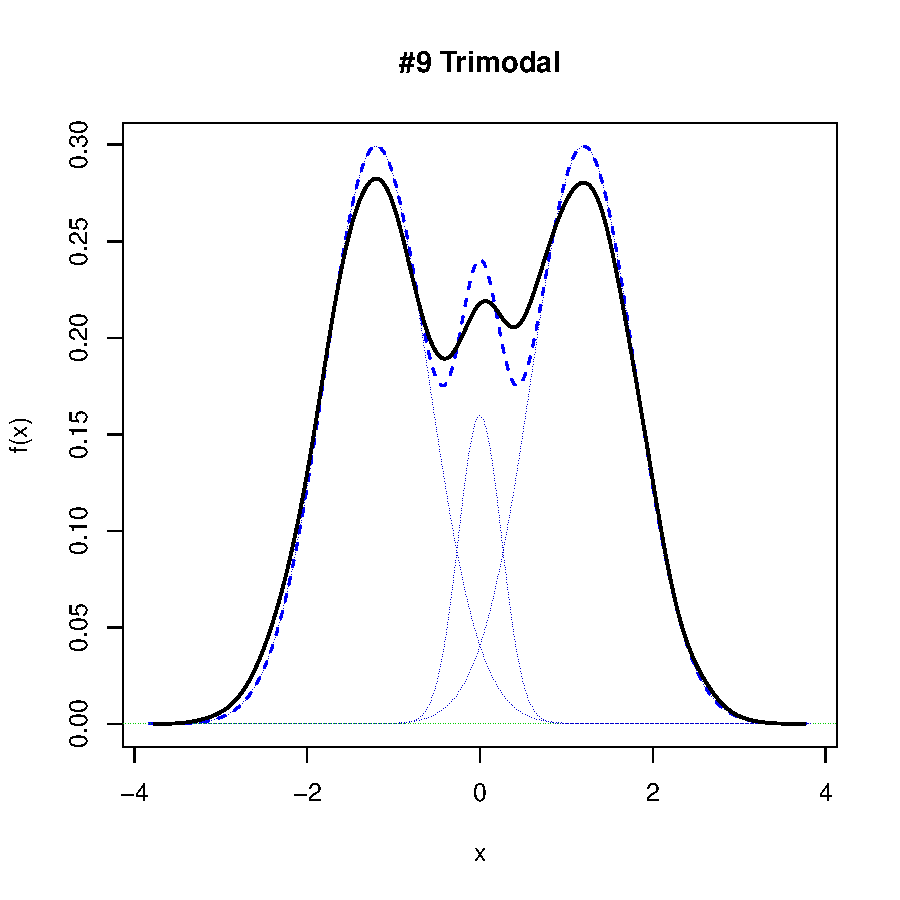
\includegraphics{chapter1-figTrimodal}
    \caption{True and estimated density of {\tt MW.nm9}}
    \label{fig:MW.nm9}
    \end{Rgraph}
\end{figure}

We can see in \ref{fig:20em}, that the EM-algorithm seems to converge to an 
intermediary solution, where the smaller middle solution is weighted lower, 
until it manages to correct back and find the correct components.



\begin{figure}[h]
    \begin{Rgraph}[0.9]
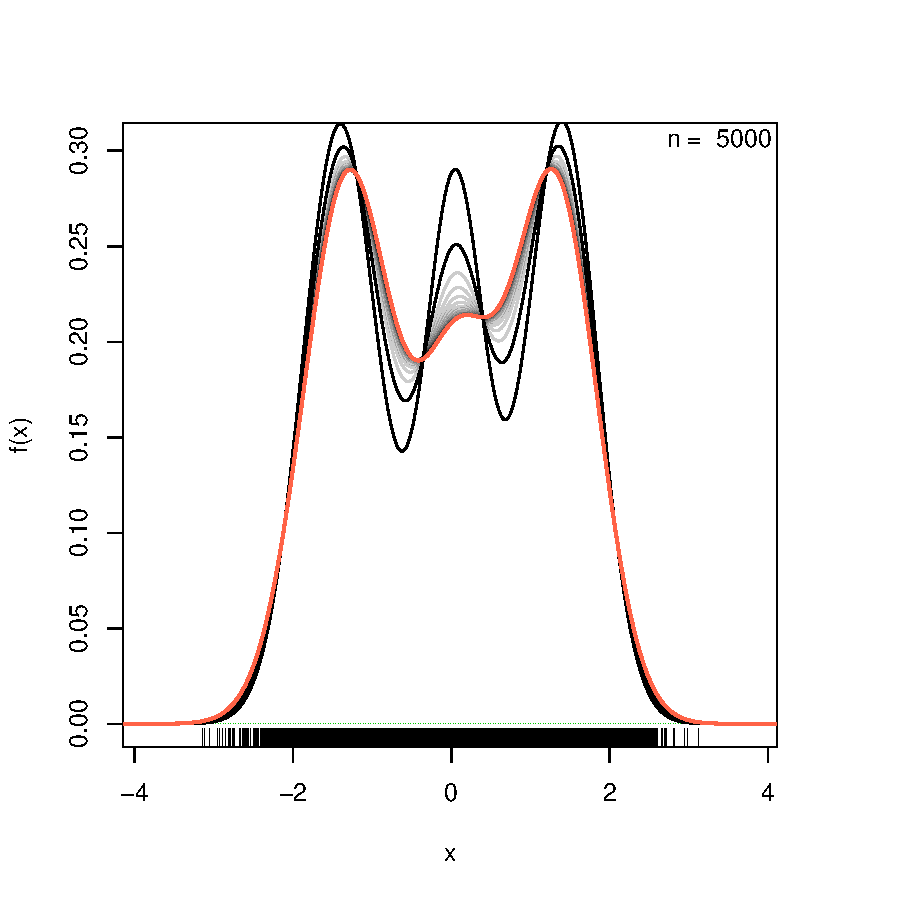
\includegraphics{chapter1-fignor1mixEx}
    \label{fig:20em}
    \caption{20 EM steps}
    \end{Rgraph}
\end{figure}

\begin{figure}[h]
    \begin{Rgraph}[0.9]
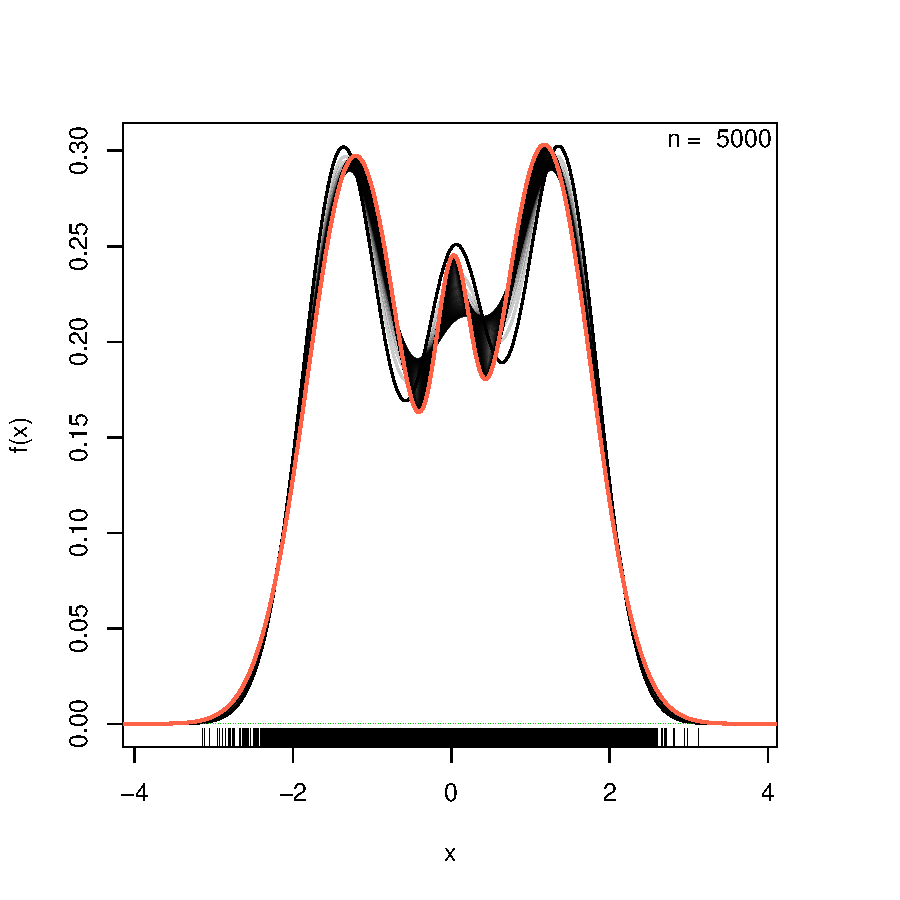
\includegraphics{chapter1-figplotemsteps}
    \label{fig:200em}
    \caption{200 EM steps}
    \end{Rgraph}
\end{figure}

We see how change in log-likelihood seems to stagnate. However, this does not 
stay that way. If we let EM run a bit further we see in figure \ref{fig:emll}, the log-likelihood hits 
a flatspot, after which convergence accelerates again.

\begin{figure}[h]
    \begin{Rgraph}[0.9]
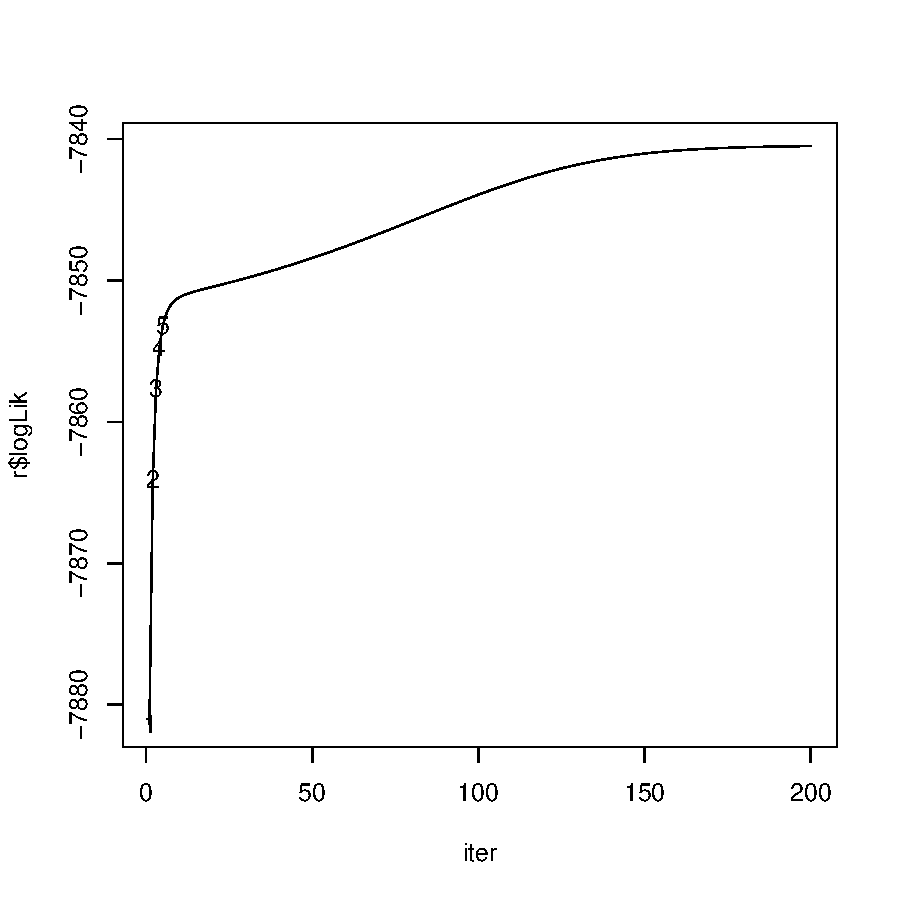
\includegraphics{chapter1-figemll}
    \label{fig:emll}
    \caption{Log-likelihood plotted against iteration count for the example in 
             \ref{fig:200em}}
    \end{Rgraph}
\end{figure}

In fact, it seems that the previous solution is a saddle point in the likelihood
function, where EM has chronic problems continuing improvements.

\chapter{The {\tt norMmix} Package}


\section{Introduction to the {\tt norMmix} Package}
\label{sec:nMm}

For this thesis, an \Rp package was developed that implements an algorithm
that fits multivariate normal mixtures to given data.
\footnote{The package was written with \Rp version 3.6.1 (2019-07-05) last 
updated on 2019-10-22.}

The algorithm is reasonably straightforward:

\begin{enumerate}
    \item Initialize using a common clustering algorithm.
    \item Perform one m-step, to transform clustering results into the form of a
        normal mixture.
    \item Apply a general optimizer, using the mixture's log-likelihood function.
\end{enumerate}

The {\tt norMmix} package is constructed around the {\tt norMmix} object that 
codifies a {\tt nor}mal {\tt M}ultivariate {\tt mix}ture model,  and the {\tt 
llnorMmix()} function, that calculates the log-likelihood given a model and 
data.

In the table \ref{tab:code-notation} the notation used in code is listed
along with a translation to the previously used mathematical notation.
Additionally, functions with ambiguous names are listed here.

\begin{table}
    \centering
    \begin{tabular}{l l}
        \hline
        In Notation & In Code \\
        \hline
        $\pi_i$     & {\tt w, weights} \\
        $\Sigma$    & {\tt Sigma} \\
        $\mu$       & {\tt mu} \\
        $K$         & {\tt k} \\
        dimension   & {\tt p, dim, dims} \\
        components  & {\tt cl, components} \\
        $\pmb{\Sigma}$ model & {\tt model} \\
        {\tt cluster}'s CLARA & {\tt clara} \\
        {\tt mclust}'s hierarchical clustering & {\tt mclVVV} \\
        {\tt mclust}'s {\tt Mclust} function & {\tt mclust} \\
        \hline
    \end{tabular}
    \caption{Translation Table: Mathematical Notation to \Rp Code}
    \label{tab:code-notation}
\end{table}


% it 1
The package contains the following functionality:
\begin{table}
\begin{description}
    \item [norMmix] {\tt norMmix()} is the 'init-method' for 
        {\tt norMmix} objects. There exist {\tt is.norMmix} {\tt rnorMmix} and
        {\tt dnorMmix} functions.
    \item [parametrization] The main functions that handle reparametrization
        of models from and to the $\pmb{LDL}^\top$ decomposition are 
        {\tt nMm2par} and {\tt par2nMm}, which are inverse to each other.
    \item [MLE] The function {\tt norMmixMLE} marries the main components of 
        this package. It initializes a model and parametrizes it for use with 
        {\tt optim}
    \item [model choice] Using {\tt norMmixMLE}, the function fitnMm allows 
        fitting of multiple models and components. Functions analyzing the 
        output of this are also provided, e.g. {\tt BIC} and {\tt print} methods.
    \item [example objects] Following the paper of \cite{Mar92} various example
        objects are provided and used for study. They follow the naming 
        convention: MW + dimension + number. For example {\tt MW213} for the 
        13th model of dimension 2.
    \item [simulations] A good portion of the package is designed with the study 
        of simulations in mind. Therefore there are functions provided to study 
        large collections of evaluated data. e.g {\tt compplot}
    \item [misc] There are also various methods of generics, like {\tt logLik,
        print, BIC, AIC} and {\tt nobs} as well as various {\tt print} methods.
\end{description}
\end{table}

The package relies on {\tt optim} from the {\tt stats} package \cite{sta19} 
for general optimization. We use the standard method implemented in {\tt optim} 
which is {\tt BFGS}, which is a quasi-Newton method (also known as a variable 
metric algorithm) as described in \cite{Bro70} among others. 

The workflow when using the package is as follows.
The function {\tt rnorMmix} can be used to generate data from a {\tt norMmix} 
object. The {\tt MW} objects provide ready made examples and objects of study
and the {\tt norMmix} function can be used to define normal mixtures from 
scratch. Of course, other data sets can be used for analysis. The following 
functions rely, however, on the {\tt matrix} data structure. So data frames 
must be converted beforehand and non numerical data is not accepted.

The functions that accept it for analysis are mainly {\tt norMmixMLE} and 
{\tt fitnMm}. The former performs model fit on data, and the latter performs 
model selection, by calling {\tt norMmixMLE} for specified {\tt k} and 
{\tt model} vectors. 

\subsection{{\tt norMmixMLE}}

The core of {\tt norMmixMLE} is the application of {\tt optim} in conjunction
with {\tt llnorMmix} as function to be optimized. {\tt llnorMmix} can be 
accessed directly, however, it needs a transposed dataset.
The {\tt norMmixMLE} function implicitly performs initialization.

There are two options for this initialization step. One is the CLARA clustering
algoritm, with non-standard arguments. The standard arguments are somewhat 
historic in origin and were, at the time, chosen because of hardware 
limitations. The arguments used in this work are defined by a function, due to 
this thesis' advisor Martin M\"achler, which was designed to be a 'sensible' 
alternative, but should be subject to further scrutiny. It is reproduced here.

\begin{Schunk}
\begin{Sinput}
>     norMmix:::ssClaraL
\end{Sinput}
\begin{Soutput}
function (n, k, p) 
pmin(n, pmax(40, round(10 * log(n))) + round(2 * k * pmax(1, 
    log(n * p))))
<bytecode: 0x45358d8>
<environment: namespace:norMmix>
\end{Soutput}
\end{Schunk}

It is dependent on the size and dimension of the dataset, as well as the 
demanded number of clusters.

The alternative to CLARA is {\tt mclust}'s hierarchical agglomerative 
clustering, which follows the work of \cite{Fra98}. The intention behind using 
{\tt mclust}'s initialization function is to directly compare how much 
difference the initialization process makes.

The initialization stage does not yield a normal mixture. This requires a way
to transform a clustering into a mixture. The method chosen in this package is
to use an m-step from the EM-algorithm. Unlike the EM-algorithm, clustering 
algorithms like CLARA produce binary cluster membership results, whereas the 
component membership of EM is determined as a probability value between 0 and 1.
This is resolved by interpreting the results as probability values which are 
either 0 or 1. These are then used as the $\tau_j$ as described in section 
\ref{sec:sketch}. This m-step is also taken from the {\tt mclust} package for 
reasons better explained in section \ref{sec:devel}.
It has the advantage of being able to generate a mixture object with the 
correct covariance model.

This mixture object is still in human readable form and not the necessary 
parameter vector demanded by {\tt optim}. So an application of the function
{\tt nMm2par} is carried out, resulting in a starting value for {\tt optim}.

The returned results from {\tt norMmixMLE} are more than abundant. Not only is 
the fitted model returned but also everything produced by {\tt optim} and the 
entire dataset. Here the return values are listed:

\begin{Schunk}
\begin{Sinput}
>     data(fSMI.12, package="norMmix")
>     str(fSMI.12$nMm[3,3][[1]], max=2)
\end{Sinput}
\begin{Soutput}
List of 6
 $ norMmix:List of 6
  ..$ mu    : num [1:20, 1:3] 15.9 30.7 36.2 21.8 753 ...
  ..$ Sigma : num [1:20, 1:20, 1:3] 0.358 0 0 0 0 ...
  ..$ weight: num [1:3] 0.219 0.419 0.362
  ..$ k     : int 3
  ..$ dim   : int 20
  ..$ model : chr "EEI"
  ..- attr(*, "name")= chr "model = EEI , clusters = 3"
  ..- attr(*, "class")= chr "norMmix"
 $ optr   :List of 5
  ..$ par        : num [1:82] 0.264 0.118 15.903 30.67 36.155 ...
  ..$ value      : num 7370
  ..$ counts     : Named int [1:2] 232 88
  .. ..- attr(*, "names")= chr [1:2] "function" "gradient"
  ..$ convergence: int 0
  ..$ message    : NULL
 $ npar   : int 82
 $ n      : int 141
 $ x      : num [1:141, 1:20] 16.1 15.7 15.7 16.1 16.6 ...
  ..- attr(*, "dimnames")=List of 2
 $ cond   : num 1.72
 - attr(*, "class")= chr "norMmixMLE"
\end{Soutput}
\end{Schunk}

Besides {\tt mclust} and {\tt cluster}, the package also relies on a number of other packages for 
various tasks. Listed in no particular order: 
{\tt MASS} \cite{mas02}, 
{\tt mvtnorm} \cite{mvt19}, 
{\tt mixtools} \cite{mix09} and 
{\tt sfsmisc} \cite{sfs19}.


\section{On The Development of {\tt norMmix}}
\label{sec:devel}

During the development of the {\tt norMmix} package several mistakes were made
and dead-ends were reached. In the interest of documentation, we discuss some
of them in this section. 

One dead-end was the parametrization of the weights of a mixture using the 
{\tt logit} function.

\begin{Schunk}
\begin{Sinput}
> logit <- function(e) {
+     stopifnot(is.numeric(e) ,all(e >= 0), all.equal(sum(e),1))
+     qlogis(e[-1L])
+ }
> logitinv <- function(e) {
+     if (length(e)==0) {return(c(1))}
+     stopifnot(is.numeric(e))
+     e<- plogis(e)
+     sp. <- sum(e)
+     w <- c((1-sp.), e)
+ }
\end{Sinput}
\end{Schunk}

This uses the logistical function {\tt logis} to transform to reduce the number
of weights from $K$ to $K-1$. Much like {\tt clr1}, given a list of weights 
{\tt logit} will transform them and {\tt logitinv} will correctly reverse the 
transformation. However, unlike {\tt clr1}, it will not transform an arbitrary 
list of length $K-1$ into a valid weight parameter. For example:

\begin{Schunk}
\begin{Sinput}
> w <- runif(7); ret <- logitinv(w)
> ret
\end{Sinput}
\begin{Soutput}
[1] -3.1906158  0.6511258  0.5136217  0.5337424  0.5794803  0.6053432  0.5846750
[8]  0.7226274
\end{Soutput}
\end{Schunk}

The issue here is that the last line of {\tt logitinv}, which is necessary to 
sum to one, but results in a negative value in {\tt ret[1]} which is not a 
valid weight. The underlying issue is that not every tuple in $\R^{K-1}$ is 
a result of {\tt logit}.

The option to use {\tt logit} is still an argument to {\tt norMmixMLE} by 
specifying {\tt trafo="logit"}, but it shouldn't be used.

Another issue during development cropped up during fitting of high dimensional
data. We studied the dataset {\tt SMI.12} from the package {\tt copula}, 
\cite{cop18}:

\begin{Schunk}
\begin{Sinput}
> data(SMI.12, package="copula")
> str(SMI.12)
\end{Sinput}
\begin{Soutput}
 num [1:141, 1:20] 16.1 15.7 15.7 16.1 16.6 ...
 - attr(*, "dimnames")=List of 2
  ..$ : chr [1:141] "2011-09-09" "2011-09-12" "2011-09-13" "2011-09-14" ...
  ..$ : chr [1:20] "ABBN" "ATLN" "ADEN" "CSGN" ...
\end{Soutput}
\end{Schunk}

A consequence of high dimensions is that matrix multiplication is no longer
very stable. As a result, the covariance matrices produced by our own 
implementation of the EM-algorithms m-step ({\tt mstep.nMm}) were not positive
definite.
In the case of {\tt SMI.12}, several covariance matrices are degenerate, which
results in cancellation error with near-zero entries.
We attempted to correct this with the function {\tt forcePositive}, which 
simply tries to set $\pmb{D}$ in $\pmb{LDL}^\top$ greater than zero.
This didn't resolve the issue, since a non-negligible part of the numerical
error was in the $\pmb{L}$ matrix and the resultant covariance matrix was still
not positive definite.

We eventually resolved this issue by abandoning our own implementation and 
using the functions from the {\tt Mclust} package. Not only were these 
numerically stable they were also able to differentiate between models, whereas
ours would assume VVV for every fit.


\section{Demonstration}
\label{sec:demo}

To end this chapter, here a small demonstration of the capabilities of 
{\tt norMmix}. First a small plot to show an MW mixture.

\begin{figure}
    \begin{Rgraph}[0.9]
\begin{Schunk}
\begin{Sinput}
>     plot(MW215)
\end{Sinput}
\end{Schunk}
    \caption{Demonstration of the MW object {\tt MW215}. Correct model: 
             {\tt model="VEE", k=3}.}
    \label{fig:demoMW}
    \end{Rgraph}
\end{figure}

It is a trimodal mixture along the diagonal.

The results of a run of {\tt norMmixMLE} are shown along with a plot of the 
fitted mixture overlaid over the correct mixture in figure \ref{fig:democorfit}.

\begin{Schunk}
\begin{Sinput}
>     set.seed(2019); x <- rnorMmix(500, MW215)
>     system.time(mleResult <- norMmixMLE(x, 3, "VEE"))
\end{Sinput}
\begin{Soutput}
initial  value 2206.907425 
iter  10 value 2147.633703
iter  20 value 2125.658743
final  value 2125.658364 
converged
   user  system elapsed 
  0.256   0.012   0.266 
\end{Soutput}
\begin{Sinput}
>     mleResult
\end{Sinput}
\begin{Soutput}
object of class 'norMmixMLE' 
norMmix object: 
multivariate normal mixture model with the following attributes:
name: 		 model = VEE , components = 3 
 model: 		 VEE 
 dimension:	 2 
 components:	 3 
weight of components 0.365 0.325 0.31 

returned from optim:
function gradient 
      75       22 

log-likelihood: -2125.658 
 
 nobs	npar	nobs/npar
 500 	 13 	 38.46154 
\end{Soutput}
\end{Schunk}

\begin{figure}[h]
    \begin{Rgraph}[0.9]
\begin{Schunk}
\begin{Sinput}
>     op <- par(mfrow=c(1,2), mar=c(1,2,3,1))
>     plot(MW215, asp=1, ylab='', xlab='')
>     points(x, col=adjustcolor("black", 0.5))
>     plot(MW215, asp=1, ylab='', xlab='')
>     plot(mleResult, fillcolor=norMmix:::nMmcols[2], newWindow=FALSE, points=FALSE)
>     legend("bottomright", legend=c("correct", "fitted"),
+            fill=norMmix:::nMmcols[1:2])
>     par(op)
\end{Sinput}
\end{Schunk}
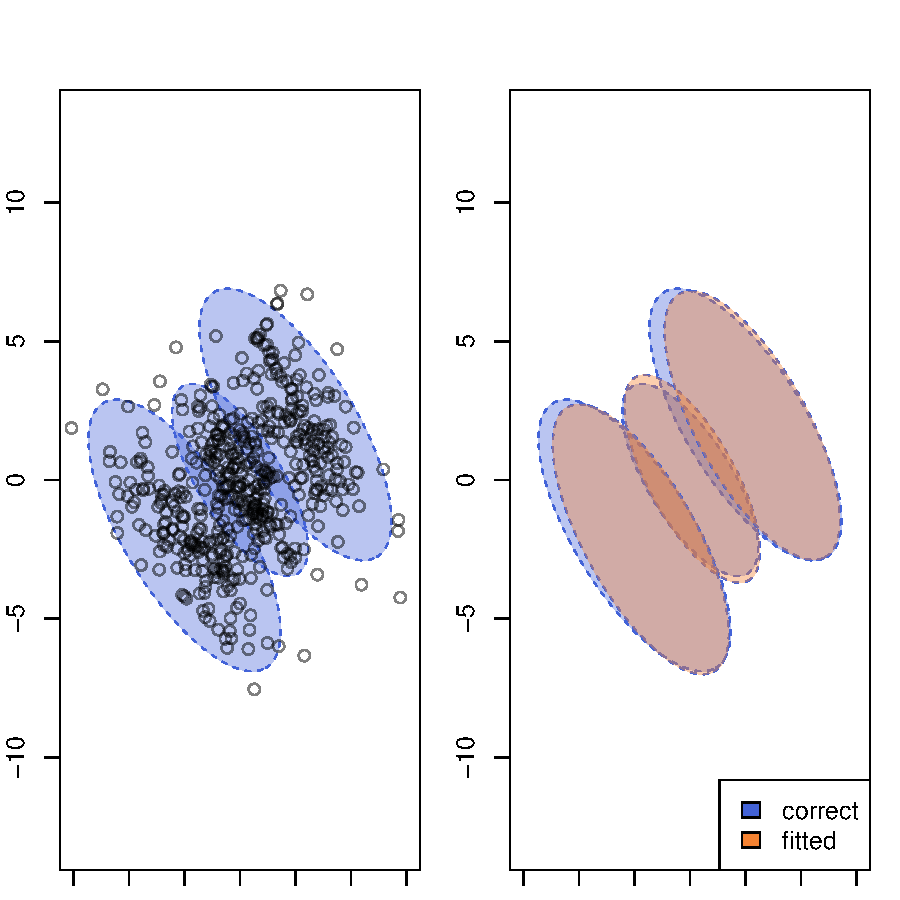
\includegraphics{chapter2-testtt}
    \caption{Correct Mixture (left) and Fitted overlayed in orange (right)}
    \label{fig:democorfit}
    \end{Rgraph}
\end{figure}

\chapter{Comparing Algorithms}


% it 1
With the {\tt norMmix} package explained, we can turn to comparing it to 
existing methods. As previously stated, the implementation representing the 
EM-algorithm is the {\tt mclust} package. It will be used with very little 
deviation from out-of-the-box settings, safe for restriction of the covariance 
models. This is done, so we can compare like with like.
The specific command that performs the EM-algorithm is:

\begin{Schunk}
\begin{Sinput}
>     mclust::Mclust(x, G=cl, modelNames=mo)$BIC
\end{Sinput}
\end{Schunk}

Where {\tt cl} is a vector of integers of however many components we are trying 
to fit and {\tt mo} are the model names:

\begin{Schunk}
\begin{Soutput}
 [1] "EII" "VII" "EEI" "VEI" "EVI" "VVI" "EEE" "VEE" "EVV" "VVV"
\end{Soutput}
\end{Schunk}

The {\tt \$BIC} element of the results is taken as the main tool for model 
selection, as it is advertised in the package authors paper \cite{Scr16}.

There is however a small but crucial change applied to these results.
The {\tt mclust} package authors have flipped the definition of the BIC to mean:
\begin{equation} 
    2 ln(\hat{L}) - ln(n) \#\{par\}
\end{equation}
instead of the more common
\begin{equation} 
    ln(n) \#\{par\} - 2 ln(\hat{L})
    \label{eqn:BIC}
\end{equation}
Where $n$ is the number of observations, \#\{par\} is the cardinality of the 
parameter vector and $\hat{L}$ is the estimated log-likelihood.

So, even if not explicitly mentioned, we use the negative of the values returned
by {\tt mclust}.

Another thing that should be stated before all else is the difference in 
initialization between {mclust}'s pre-clustering and CLARA. CLARA is dependent
on random number generators. As such, unless a fixed seed is chosen, every 
iteration of CLARA will return a different result. Unlike {\tt mclust}, which 
will, for given data, always return the same results. The effect on the 
following findings is that results will spread out for data obtained from 
CLARA results.

First, we illustrate the structure of the graphical results we will be 
presenting hereafter. The basic shape of the plots will be the BIC value 
plotted against the number of components. This is in line with {\tt mclust}'s
manner of visualizing data, however since our method is to some extent RNG 
dependent, we are forced to display multiple runs of the algorithm on the same
graph. Therefore we split the plot according to covariance model, putting 10
models in 10 graphs in a plot. Here an example:


\begin{figure}[h!]
    \begin{Rgraph}[0.9]
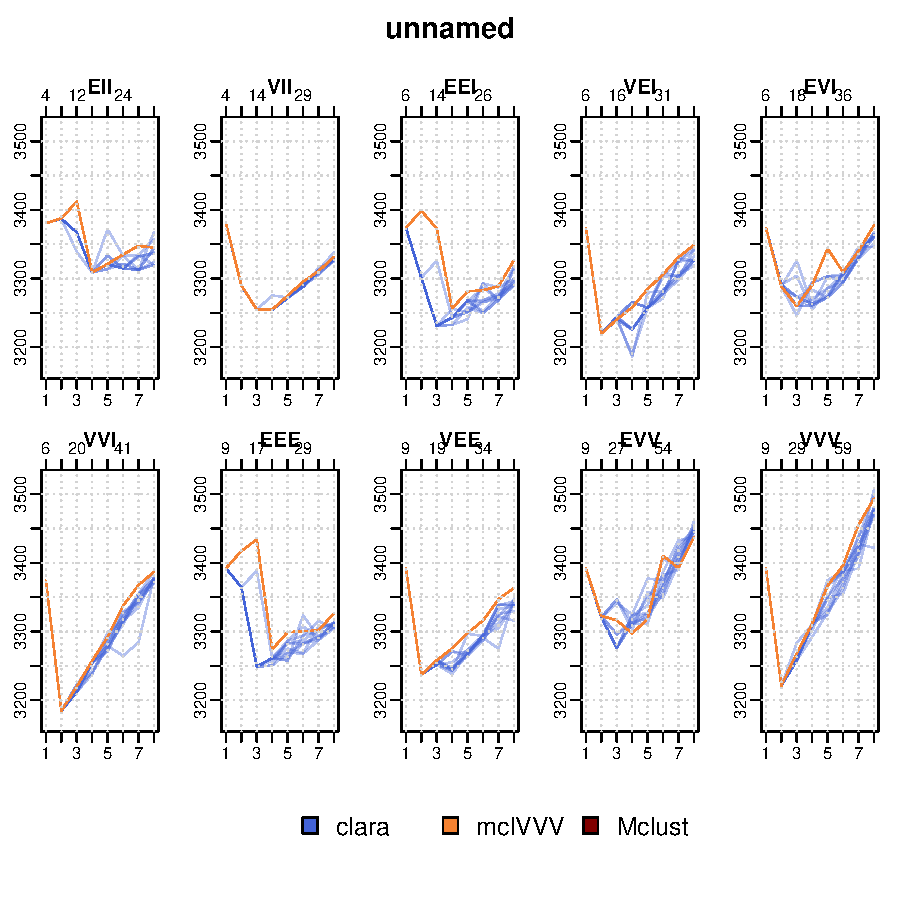
\includegraphics{chapter3-bicplotdemoplot}
    \caption{Example of comparison plot}
    \label{fig:ExPlot}
    \end{Rgraph}
\end{figure}

As can be seen from the formula of the BIC value \ref{eqn:BIC}, lower is better.
When selecting a model based on BIC, we take the model and component with the 
lowest value to be the best fitting model. Although this may not necessarily
the 'correct' model, that is, the model from which the data arises.

There are many ways in which this type of model selection might miss the 
correct model, for example by 'gluing together' multiple components into one,
or covering the dataset in a 'patchwork' of smaller components, to name a few.
We will discuss them as they arise in the following analysis of simulations.

The simulations were set up very simply. An \Rp script was written and in each
the {\tt norMmix} package is loaded, the datasets are defined and {\tt fitnMm}
was applied a number of times. An example script can be found in the appendix
\ref{App:sims}.

A few things of interest are what happens:

\begin{itemize}
    \item To time needed for the simulation
    \item When we vary the sample size of the data sets.
    \item When the generating mixture is 'difficult'.
    \item When the data does not arise from a normal mixture.
\end{itemize}

The data used here should have been provided along with this thesis in digital 
form in a folder called {\tt /simulations}, with individual simulations in 
their own subfolder.


\section{Time Analysis}
\label{sec:time}

The data used here is taken from the subfolder {\tt /simulations/2time}.
In this simulation we take several example mixtures and generate $n = \{500, 1000, 2000\}$.
We apply {\tt fitnMm} with {\tt clara} using ten different seeds and {\tt mclVVV}
initializations, and {\tt Mclust}.
From these, the system time was extracted and analyzed as can be gleaned from
the following code. In it, we apply \Rp's {\tt lm} function for fitting linear 
models to the times returned by the function call:

\begin{Schunk}
\begin{Sinput}
>     system.time(norMmixMLE(x, ...))[[1]]
\end{Sinput}
\end{Schunk}

We make here a choice that does not preserve any generality, as 
{\tt system.time} produces more results, that could hold important information.
However, since there is quite some measurement error to be expected as time 
approaches zero, we will content ourselves with lower expectations to the 
accuracy of the following results.


\begin{Schunk}
\begin{Sinput}
>     library(norMmix, lib.loc="~/ethz/BA/norMmix.Rcheck/")
>     # change this dir to whereever the simulations are saved
>     mainsav <- normalizePath("~/ethz/BA/Rscripts/")
>     savdir <- file.path(mainsav, "2time")
>     filelist <- list.files(savdir, pattern=".rds")
>     filelist <- grep("mcl.rds", filelist, invert=TRUE, value=TRUE)
>     f <- lapply(file.path(savdir,filelist), function(j) readRDS(j)$fit)
>     times <- unlist(lapply(f, function(j) extracttimes(j)[,,1]))
>     dims <- unlist(lapply(f, function(j) attr(extracttimes(j), "p")))
>     size <- unlist(lapply(f, function(j) attr(extracttimes(j), "n")))
>     ddims <- rep(dims, each=80)
>     ssize <- rep(size, each=80)
>     pars <- unlist(lapply(f, npar))
>     r <- lm(times ~ pars + ddims + ssize)
>     summary(r)
\end{Sinput}
\begin{Soutput}
Call:
lm(formula = times ~ pars + ddims + ssize)

Residuals:
   Min     1Q Median     3Q    Max 
-86.89  -7.45  -1.55   6.30 556.32 

Coefficients:
              Estimate Std. Error t value Pr(>|t|)    
(Intercept) -1.727e+01  8.274e-01  -20.87   <2e-16 ***
pars         9.729e-01  1.056e-02   92.16   <2e-16 ***
ddims       -3.749e+00  2.216e-01  -16.92   <2e-16 ***
ssize        9.258e-03  3.887e-04   23.82   <2e-16 ***
---
Signif. codes:  0 ‘***’ 0.001 ‘**’ 0.01 ‘*’ 0.05 ‘.’ 0.1 ‘ ’ 1

Residual standard error: 21.57 on 7916 degrees of freedom
Multiple R-squared:  0.559,	Adjusted R-squared:  0.5588 
F-statistic:  3344 on 3 and 7916 DF,  p-value: < 2.2e-16
\end{Soutput}
\end{Schunk}

The necessary time appears to be well explained by the parameter count.
The purpose of this thesis is not to conduct complexity analysis, so we will
leave it at this, satisfying our curiosity with a cursory look in figure 
\ref{fig:time}, where we plot system time against parameter length.

\begin{figure}[h!]
    \begin{Rgraph}[0.9]
\begin{Schunk}
\begin{Sinput}
>     plot(times~pars, log="xy", yaxt="n", xaxt="n", type="n")
>     legend("bottomright", legend=c("MW214", "MW34","MW51"),
+            fill=nMmcols[c(3,4,2)])
>     points(times[1:(80*30)]~pars[1:(80*30)], 
+            log="xy", yaxt="n", xaxt="n", col=nMmcols[3], pch=1)
>     points(times[(80*30+1):(80*60)]~pars[(80*30+1):(80*60)]
+            , log="xy", yaxt="n", xaxt="n", col=nMmcols[4], pch=9)
>     points(times[(60*80+1):(80*90)]~pars[(60*80+1):(80*90)], 
+            log="xy", yaxt="n", xaxt="n", col=nMmcols[2], pch=8)
>     grid()
>     sfsmisc::eaxis(1)
>     sfsmisc::eaxis(2)
\end{Sinput}
\end{Schunk}
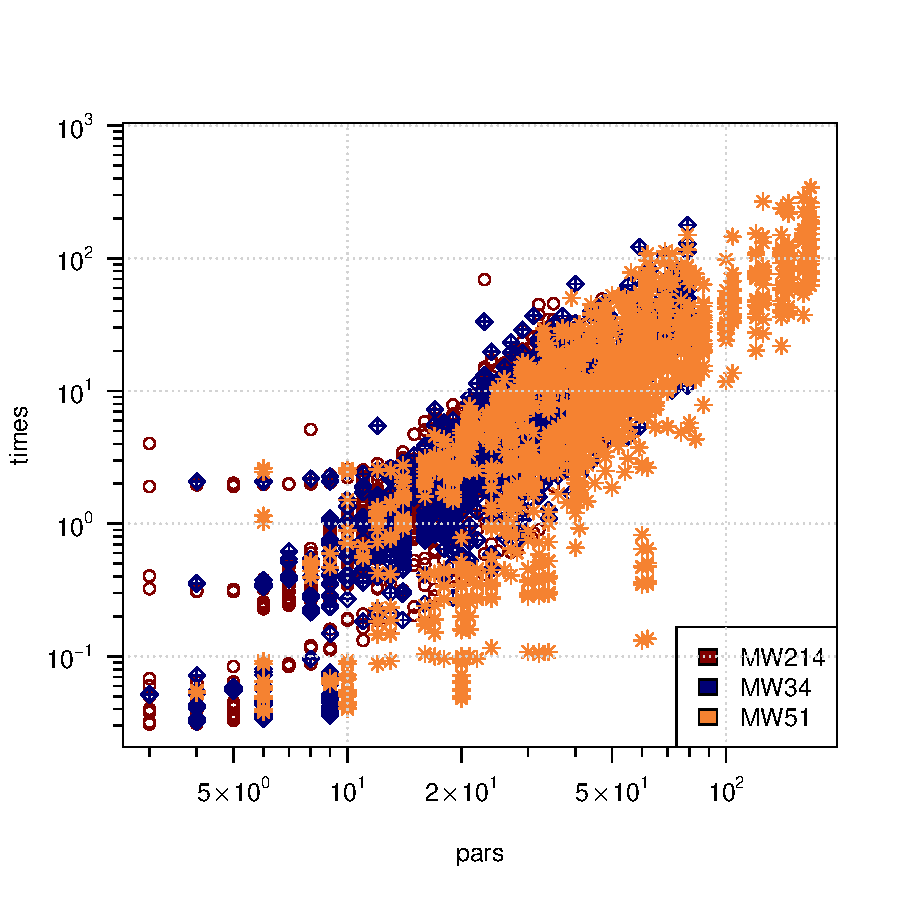
\includegraphics{chapter3-figtime}
    \caption{Log-log plot of system time against parameter length}
    \label{fig:time}
    \end{Rgraph}
\end{figure}

We can see that time is almost one to one proportional to parameter length.
It should be noted, that {\tt MW51} is a very simple mixture. It is therefore 
sensible, that MLE should find an optimum faster.

\clearpage

\section{Behaviour in {\tt n}}
\label{sec:ben}

What we would expect and like to see as we increase sample size, is a decrease
in scattering of BIC values. To that end we again use simulation data 
{\tt /simulations/2time}. In particular we show here the results of fitting to 
mixture model {\tt MW34}, shown in figure \ref{fig:MW34}. The graphs 
\ref{fig:bicmw34first} and \ref{fig:bicmw34second} show three columns
of BIC plots, each representing different sample sizes, with 
$n = \{500, 1000, 2000\}$ respectively. Furthermore, the BIC values were 
divided by the samplesize, to normalize the values to an equal scale.

\begin{figure}[h]
    \begin{Rgraph}[0.9]
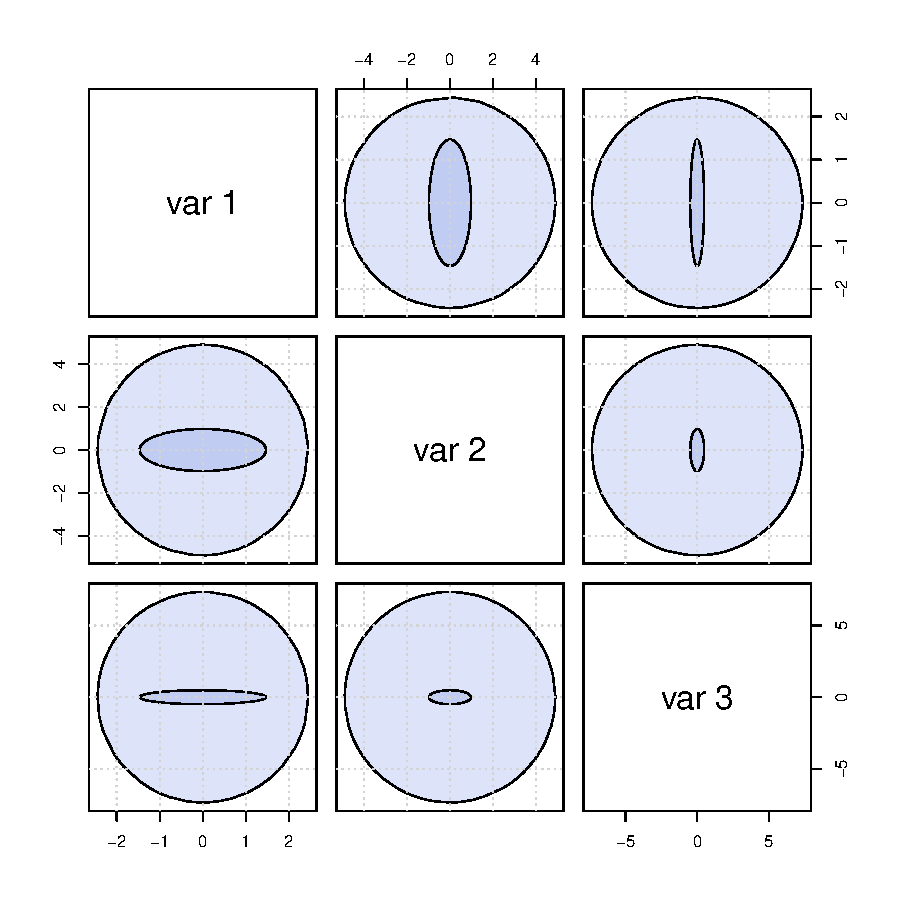
\includegraphics{chapter3-figMW34}
    \caption{The mixture model {\tt MW34}, a three dimensional, two component
             mixture with one smaller, lesser weighted component inside a 
             smaller one.}
    \label{fig:MW34}
    \end{Rgraph}
\end{figure}


\begin{figure}[h!]
    \begin{Rgraph}[0.9]
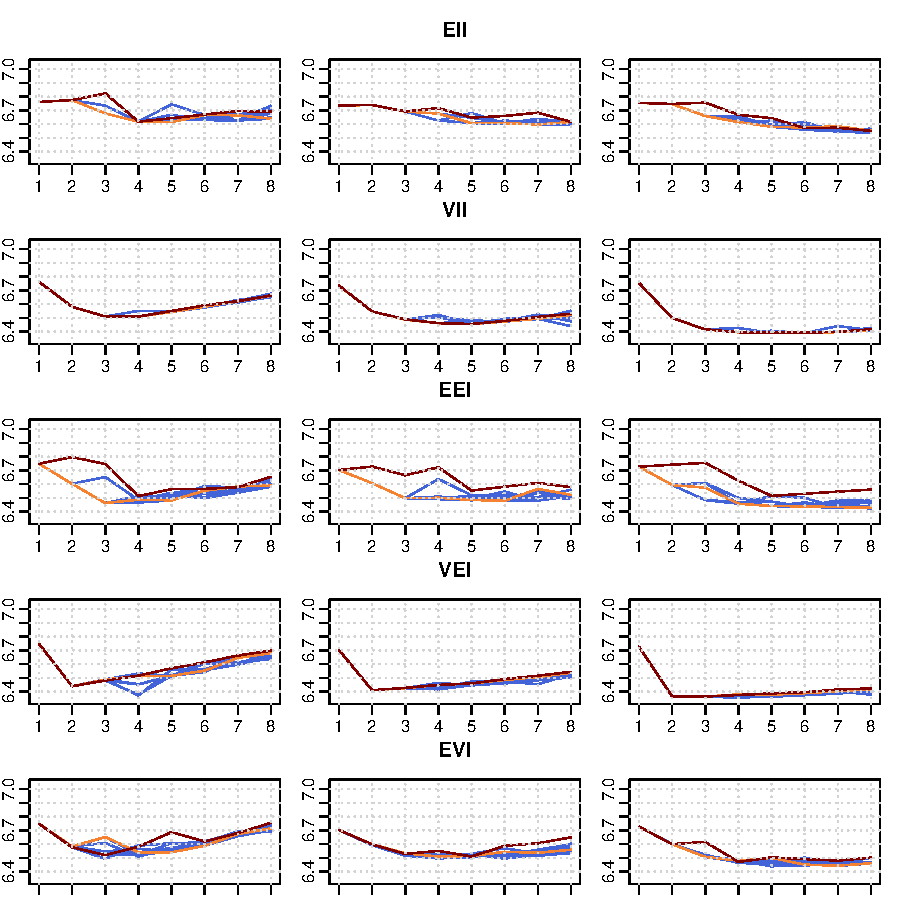
\includegraphics{chapter3-figmw34bicfirst}
    \caption{BIC values of {\tt MW34} with $n=\{500, 1000, 2000\}$. Clara was 
             applied with $10$ seeds.}
    \label{fig:bicmw34first}
    \end{Rgraph}
\end{figure}

As can be seen the desired effect is achieved. Of note are the behaviour of 
the model {\tt VEI}, where the increase in observation corrects a selection
error appearing at $n=500$. Furthermore, the correct model {\tt VVI} exhibits
a very tight grouping. The instances where {\tt mclust} is better than 
{\tt norMmix} are quite infrequent.

This type of analysis was also conducted with mixture objects {\tt MW214} and 
{\tt MW51}, but were omitted due to the lack of clear results. They are 
provided in the appendix \ref{app:ben}, with brief discussions.

\begin{figure}[h!]
    \begin{Rgraph}[0.9]
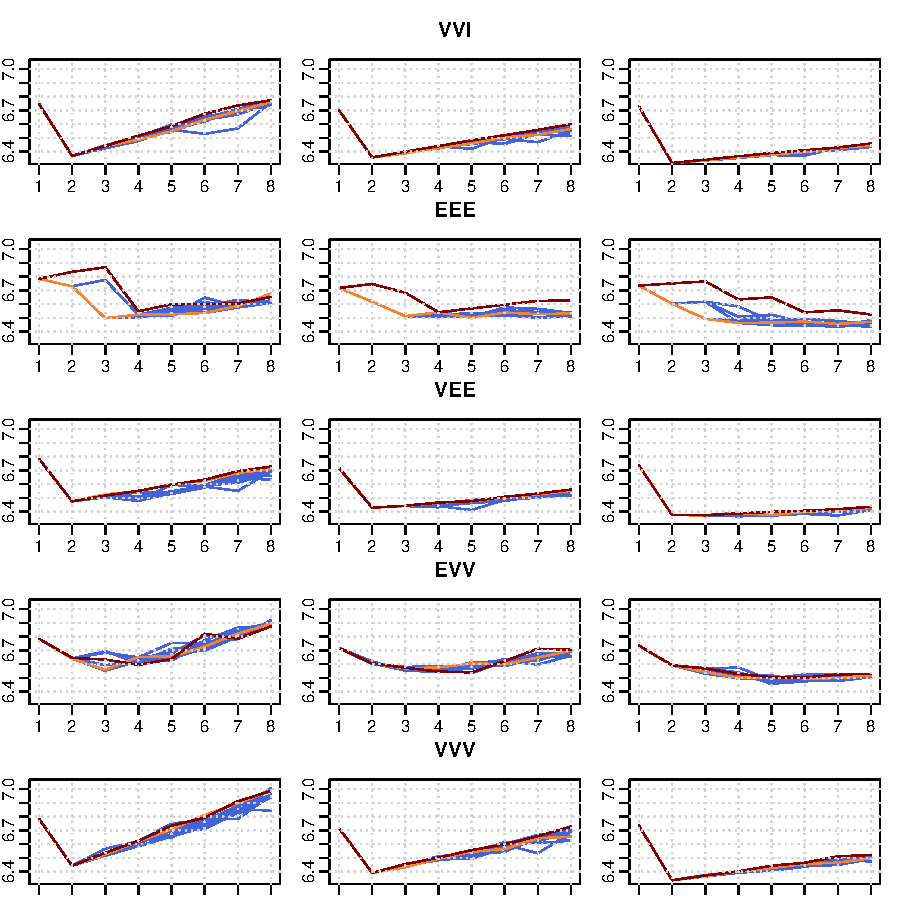
\includegraphics{chapter3-figmw34bicsecond}
    \caption{BIC values of {\tt MW34} with $n=\{500, 1000, 2000\}$. CLARA was 
             applied with 10 seeds.}
    \label{fig:bicmw34second}
    \end{Rgraph}
\end{figure}

\clearpage

\section{Difficult Mixtures}
\label{sec:dif}

In this section we analyze the two mixtures given by {\tt MW215} and {\tt MW214}.
These were generated with $n=500$ and CLARA was applied $50$ times.
These are a trimodal and a claw-like distribution. These types of mixtures were 
also discussed in \cite{Mar92}, in the univariate case, where they proved to be 
difficult to fit.

First the trimodal mixture shown in figure \ref{fig:MW215}. The difficulty 
lies in the components of various sizes lying close together.

\begin{figure}
\begin{Rgraph}[0.9]
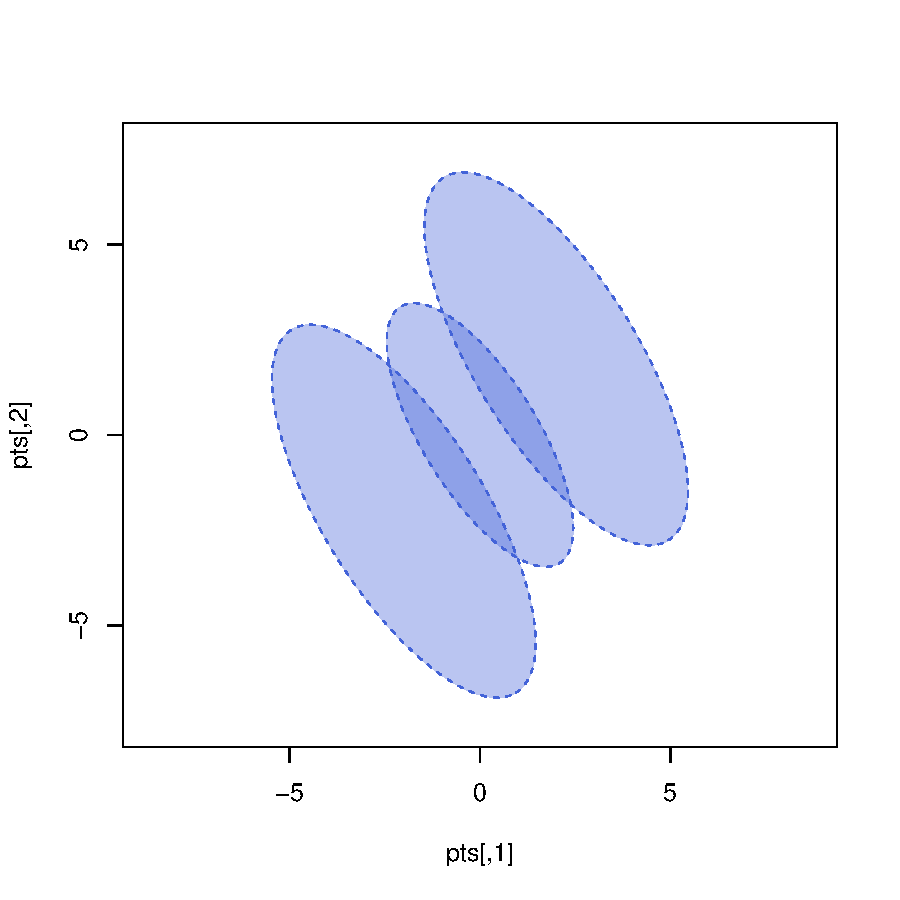
\includegraphics{chapter3-figMW215}
    \caption{Trimodal mixture {\tt MW215}. Three equally weighted, oriented, and
             shaped components of different volumes along the diagonal}
    \label{fig:MW215}
\end{Rgraph}
\end{figure}


\begin{figure}[h!]
    \begin{Rgraph}[0.9]
\begin{Schunk}
\begin{Sinput}
>     compplot(clarabic, mclbic, mclustbic, main="Fit of MW34")
\end{Sinput}
\end{Schunk}
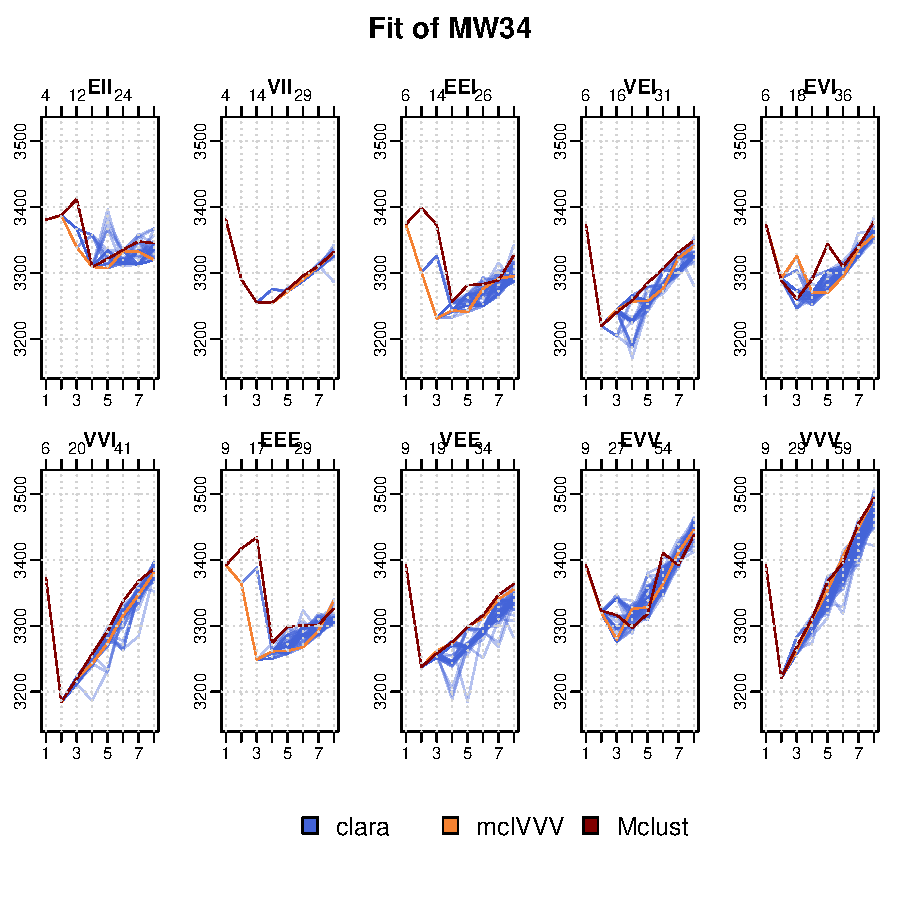
\includegraphics{chapter3-figMW34bic}
    \caption{BIC values of {\tt MW34}, correct: {\tt model="VVI", k=2}. 
             $n=500$, CLARA was applied $50$ times.}
    \label{fig:bicMW34}
    \end{Rgraph}
\end{figure}

We can see, that in many cases both initialization methods {\tt clara} and
{\tt mclVVV} manage to achieve a lower BIC value than {\tt mclust}. Although in
the case of the correct model and cluster, {\tt k=3, model="VEE"} the three 
algorithms coincide.

A search for best values reveals, that the best models selected are in almost 
all cases the correct model.

\begin{Schunk}
\begin{Soutput}
     model   count
[1,] "2 VVI" "49" 
[2,] "4 VEI" "1"  
\end{Soutput}
\end{Schunk}

The one incorrect model looks like this:

\begin{figure}[h]
    \centering
    \begin{minipage}{0.45\textwidth}
        \centering
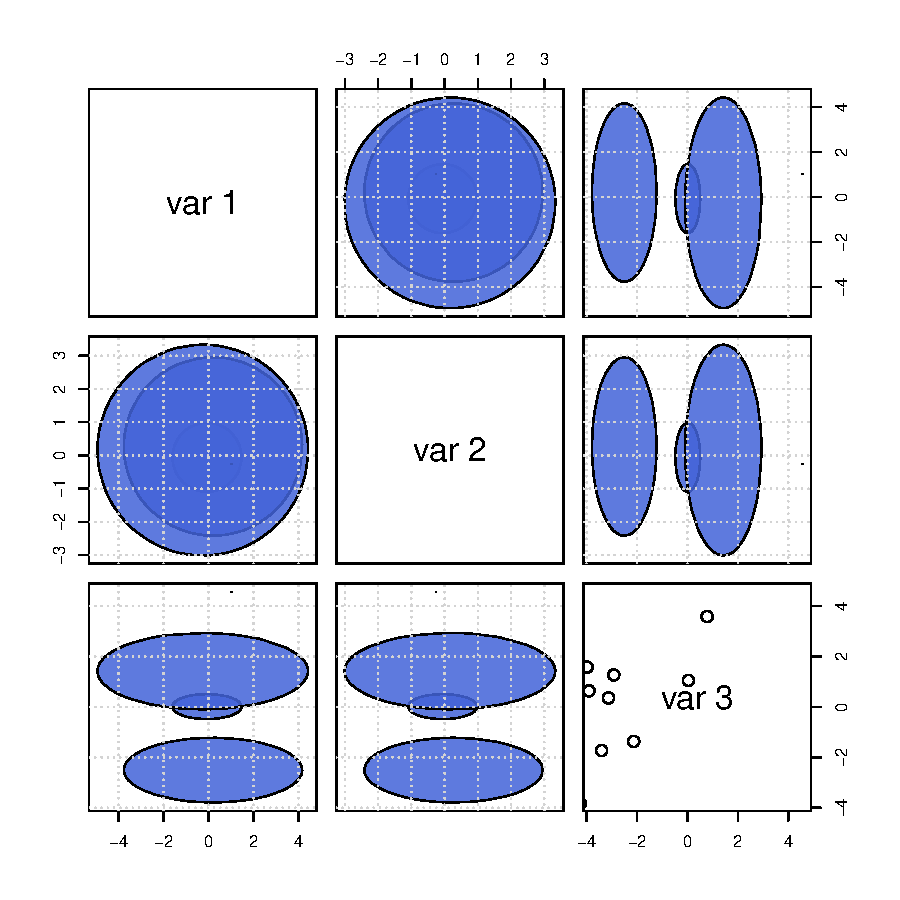
\includegraphics{chapter3-figerrorMW215}
    \end{minipage}
    \begin{minipage}{0.45\textwidth}
        \centering
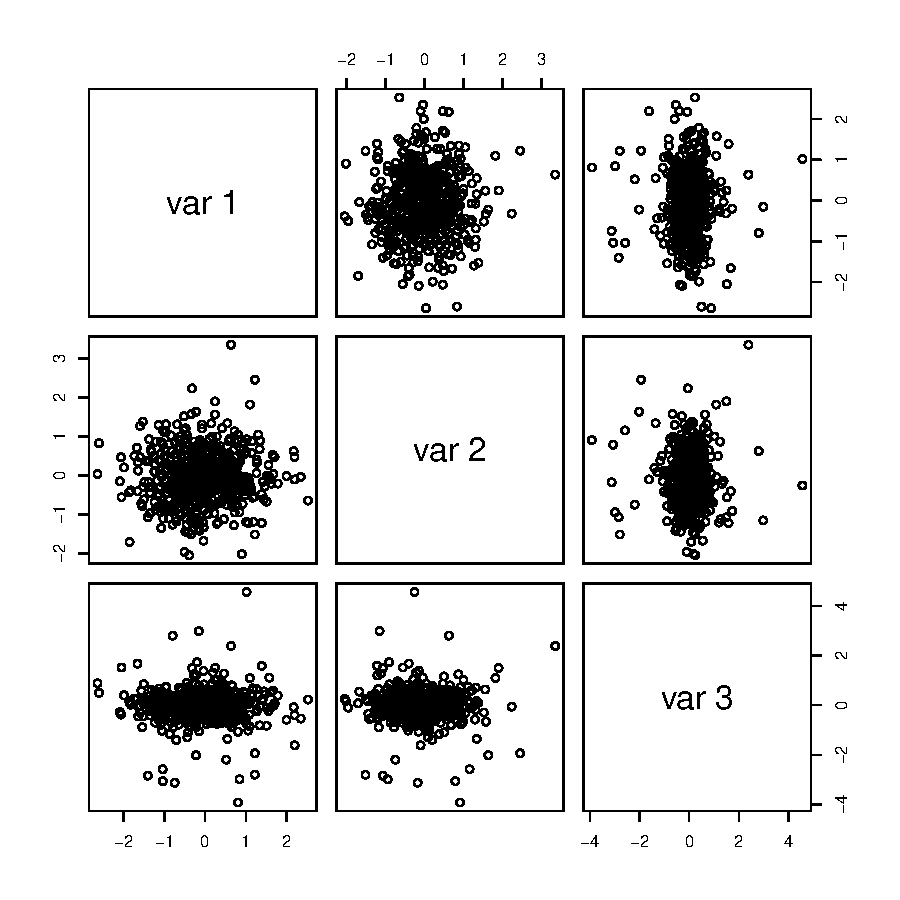
\includegraphics{chapter3-figerrorMW215x}
    \end{minipage}
\end{figure}

and has the weights: 0.942, 0.0321, 0.0244, 0.002. This is an issue of 
spurious clusters. These are clusters formed by a low number of data points
conjoined into a component with small determinant of its covariance matrix.
It is a flaw in the {\tt norMmix} package, that is not addressed.

Now for the claw-like mixture, {\tt MW214}. It is a mixture of six components
and a very simple {\tt "VII"} covariance model. A large encompassing component
and five smaller, lightly weighted components closely together along the 
diagonal. The inherent difficulty lies in the fact that the components overlap
and are close together as well. It is shown in figure \ref{fig:MW214}.

\begin{figure}[h!]
    \begin{Rgraph}[0.9]
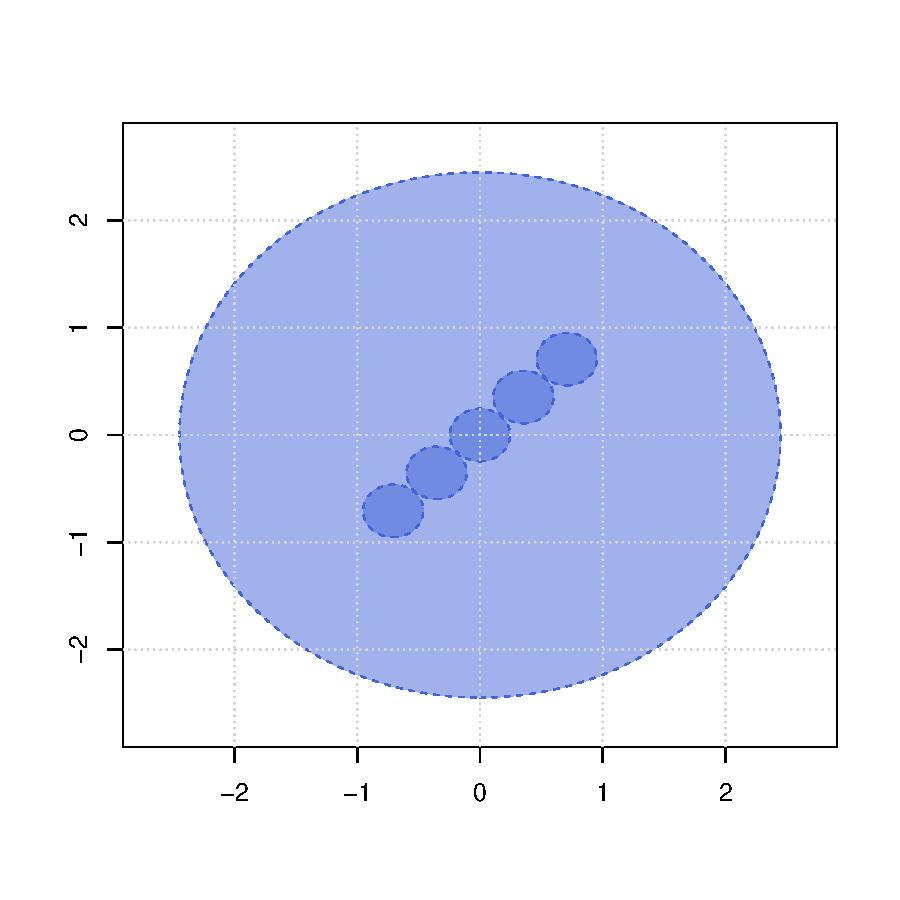
\includegraphics{chapter3-figMW214}
    \caption{Claw-like mixture {\tt MW214}}
    \label{fig:MW214}
    \end{Rgraph}
\end{figure}



\begin{figure}[h!]
    \begin{Rgraph}[0.9]
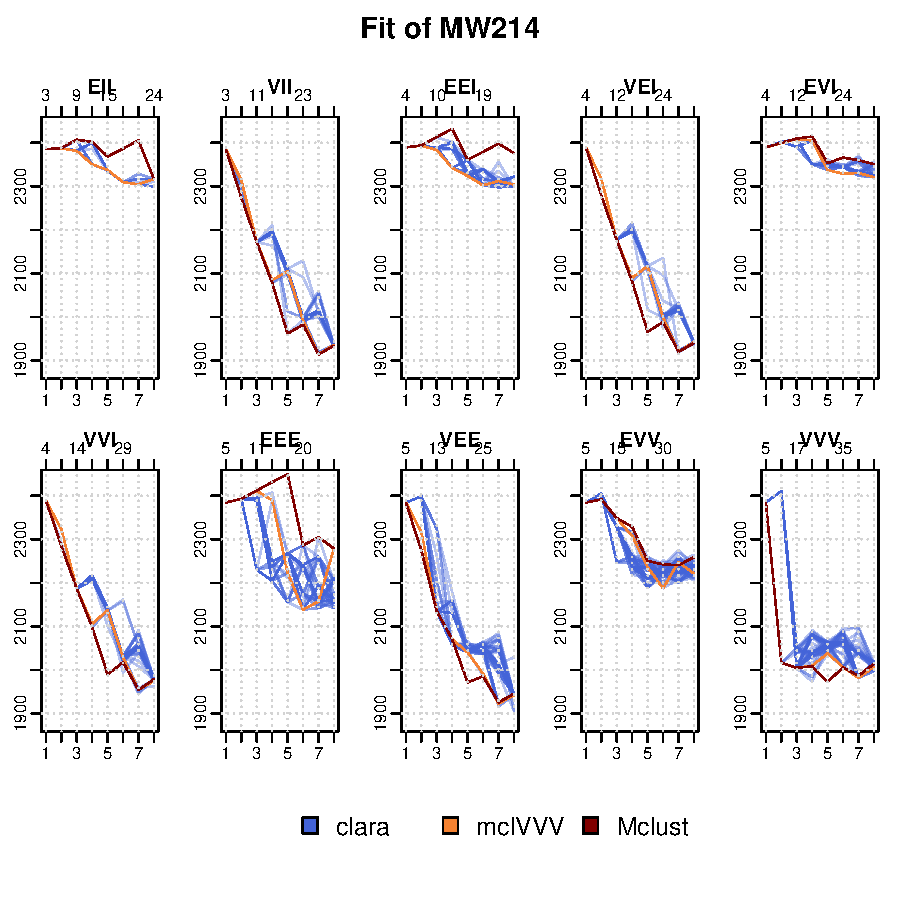
\includegraphics{chapter3-figMW214bic}
    \caption{BIC values of claw-like mixture. Best fit: {\tt model="VEE", k=8},
             correct: {model="VII", k=6}. $n=500$, CLARA was applied $50$ times.}
    \label{fig:214bis11}
    \end{Rgraph}
\end{figure}

We take a look at the best results per simulation again:

\begin{Schunk}
\begin{Soutput}
     model   count
[1,] "8 VII" "27" 
[2,] "7 VEE" "8"  
[3,] "7 VEI" "8"  
[4,] "7 VII" "4"  
[5,] "8 VEE" "3"  
\end{Soutput}
\end{Schunk}

And here are the ten best values:

\begin{Schunk}
\begin{Soutput}
      comp model BIC               
 [1,] "8"  "VEE" "1905.61014581771"
 [2,] "8"  "VEE" "1907.24944742008"
 [3,] "8"  "VEE" "1913.57109788463"
 [4,] "7"  "VII" "1913.68061849043"
 [5,] "7"  "VII" "1913.68062199219"
 [6,] "7"  "VEE" "1916.40190209225"
 [7,] "7"  "VEE" "1916.40195605402"
 [8,] "7"  "VEI" "1918.15484419568"
 [9,] "7"  "VII" "1918.35924550811"
[10,] "7"  "VII" "1918.4864952664" 
\end{Soutput}
\end{Schunk}

Here some examples of fitted mixtures:

\begin{figure}[h!]
    \begin{Rgraph}[0.9]
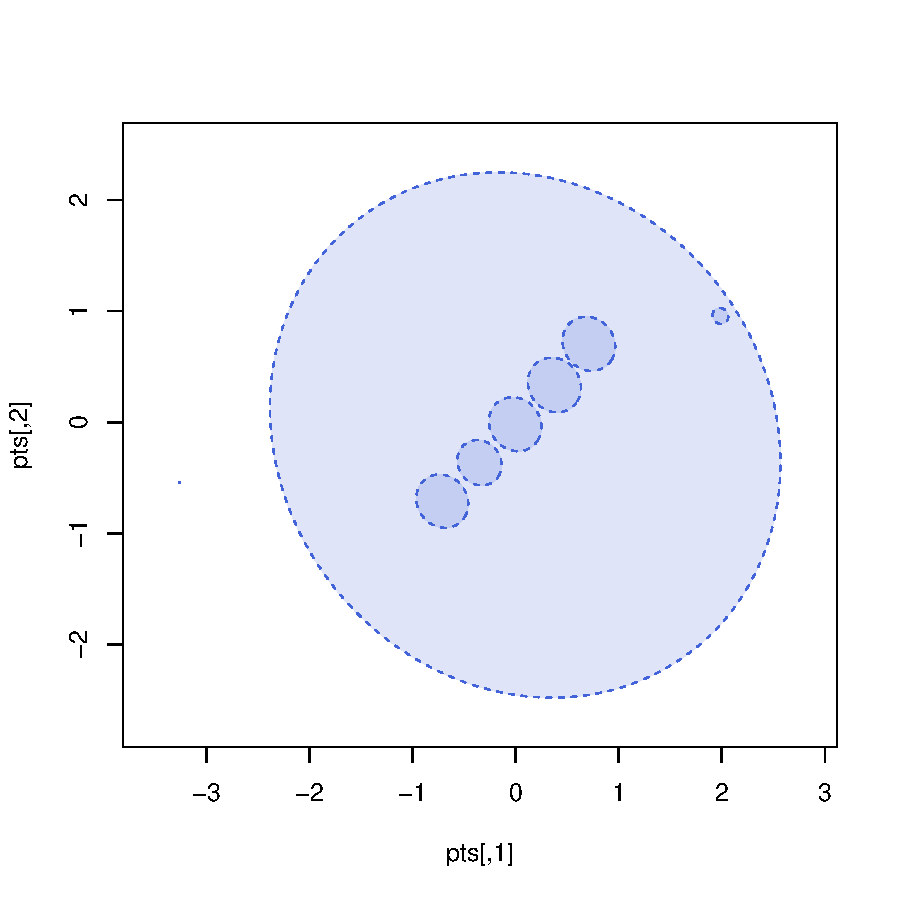
\includegraphics{chapter3-fig214fit}
    \caption{{\tt model="VEE", k=8}, correct
             model: {\tt model="VII", k=6}. Of Note Here are the Spurious 
             Clusters Appearing.}%whats n?? should be verbose
    \label{fig:MW214bestfit}
    \end{Rgraph}
\end{figure}

\begin{figure}[h]
    \begin{Rgraph}[0.9]
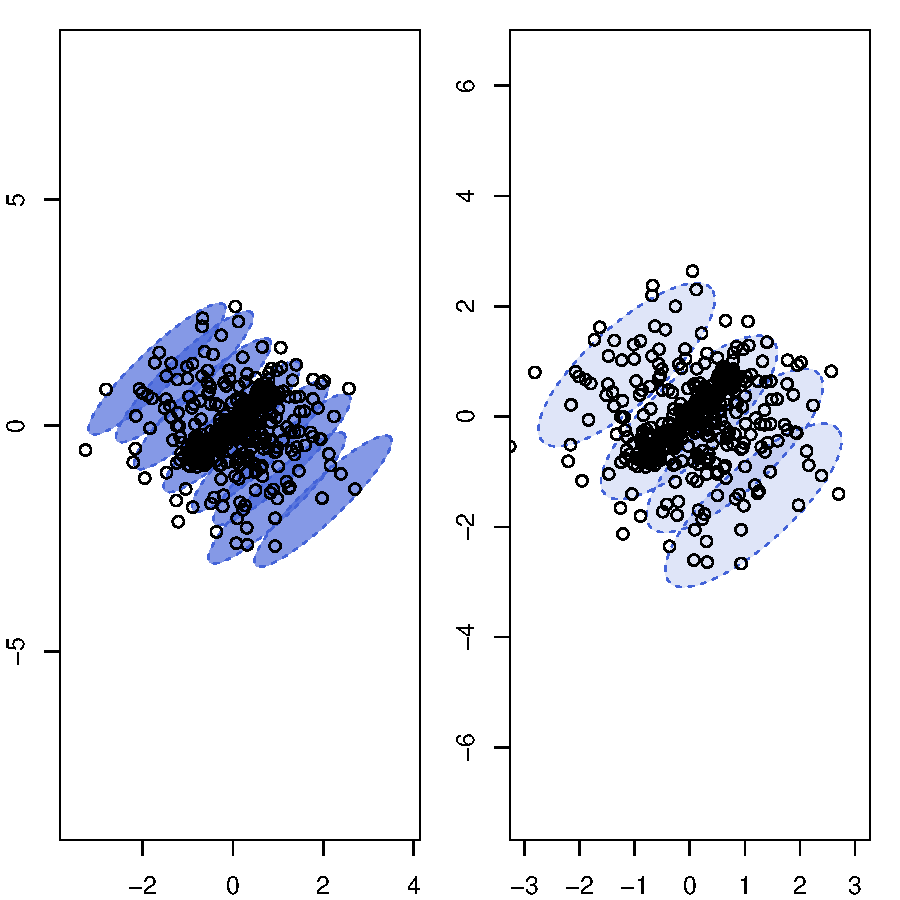
\includegraphics{chapter3-fig214fit2}
    \end{Rgraph}
    \caption{Two of the better clusters. They both follow the 'patchwork'
             covering strategy, laying patches of components over the data.}
    \label{fig:214fit2}
\end{figure}

We can see, that, subtracting the obvious hiccups of the small erroneous
components, {\tt norMmix} has correctly found the 'intended' 
distribution. This is remarkable, given the small sample size and difficulty of 
distribution. As can be seen in figure \ref{fig:214fit2}, there are mistakes in
the near best clusters, where the data is overlaid with a 'patchwork' of 
components.

\clearpage

\section{Nonnormal Mixtures}

Using only datasets generated from the intended model can hide important 
structural errors in an algorithm. To that end we also applied {\tt norMmix}
to nonnormal data to see if any erratic behaviour appears.

The data used are the {\tt SMI.12} and {\tt loss} from the package {\tt copula}
\cite{cop18}, as well as the {\tt iris} data included in base \Rp.

We begin with the {\tt SMI.12} dataset, described as "SMI.12 contains the close prices of all 20 constituents of the Swiss Market Index (SMI) from 2011-09-09 to 2012-03-28." This also doubles as high-dimensional analysis, as it is 20 dimensional.


\begin{figure}[h!]
    \begin{Rgraph}[0.9]
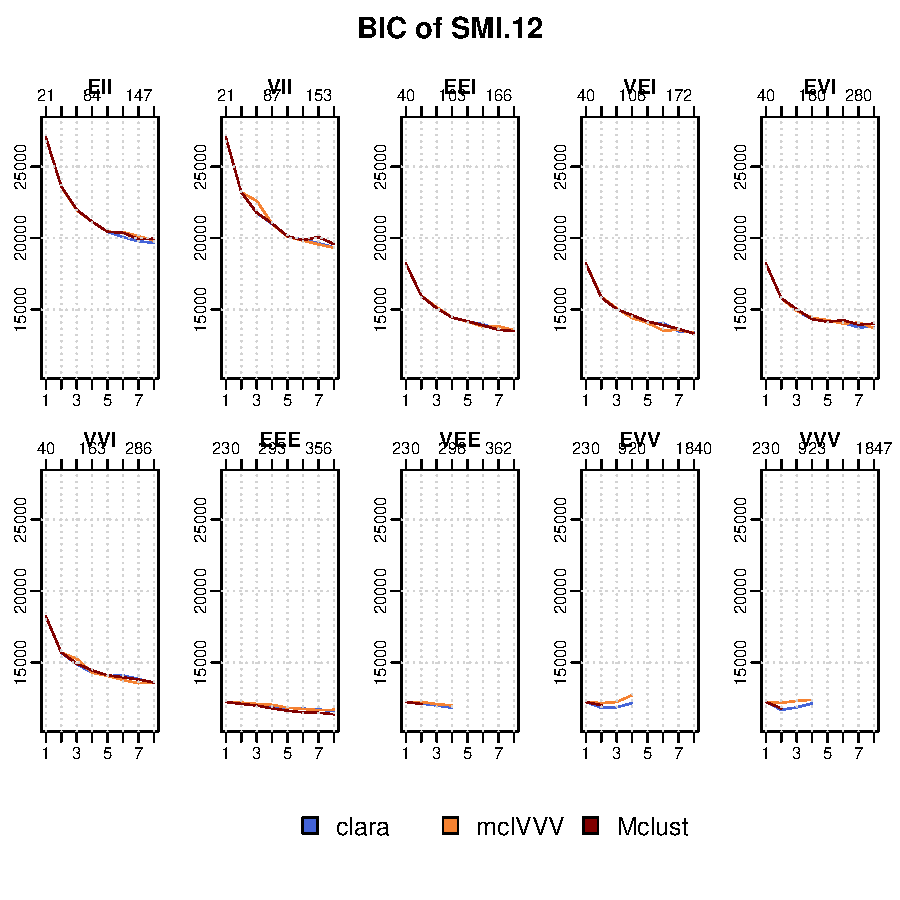
\includegraphics{chapter3-2smiplot}
    \end{Rgraph}
    \caption{The BIC values of the {\tt SMI.12} data. The blue line representing
             the {\tt clara} values is covered by the other lines. The last 
             three models are not plotted for all component sizes, as the 
             algorithm returns an error if the fitting problem is ill defined.}
    \label{}
\end{figure}

While not very spectacular, the graphs show that even at large parameter
counts our algorithm closes in on the same values as {\tt mclust}.
At these dimensions it is difficult to compare if these are actually 
equal, or even similar fits, but going by BIC values, it is at the very 
least equally viable as a working model.
The last three models are not fully plotted for all components. The reason for 
this is that {\tt norMmix} relies on {\tt mclust} in its m-step. The 
{\tt mclust} package halts computation when the clustering problem is badly 
posed. In this instance the problem is that the parameter count is much larger 
than the number of observations.

To illustrate, here are the parameter sizes for this simulation:

\begin{Schunk}
\begin{Soutput}
  EII VII EEI VEI EVI VVI EEE VEE  EVV  VVV
1  21  21  40  40  40  40 230 230  230  230
2  42  43  61  62  80  81 251 252  460  461
3  63  65  82  84 120 122 272 274  690  692
4  84  87 103 106 160 163 293 296  920  923
5 105 109 124 128 200 204 314 318 1150 1154
6 126 131 145 150 240 245 335 340 1380 1385
7 147 153 166 172 280 286 356 362 1610 1616
8 168 175 187 194 320 327 377 384 1840 1847
\end{Soutput}
\end{Schunk}

{\tt SMI.12} has 141 observations, which is exceeded by the parameter count by
all component sizes and covariance models. With a ratio of observations to 
parameters this low, it is desirable for clustering algorithms to break off and
return an error, so conclusions are not drawn from ill posed problems.

For curiosity's sake we include here the system times taken for the simulations

\begin{Schunk}
\begin{Soutput}
   models
k     EII    VII    EEI    VEI     EVI    VVI     EEE     VEE      EVV      VVV
  1 0.059  0.051  0.058  0.059   0.070  0.070   0.201   0.202    0.273    0.275
  2 0.273  0.331  1.719  1.763   4.545  3.805  61.951  59.924  224.436  232.331
  3 0.435  1.950  4.816  5.248  12.660 12.860  96.099 125.053  660.375  638.954
  4 1.384  2.456  8.715  9.145  22.173 23.065 136.370 151.448 1438.264 1556.838
  5 1.869  3.289 13.293 14.703  26.584 28.580 218.786   0.683    0.690    0.682
  6 2.703  4.125 20.578 20.490  45.355 41.667 256.036   0.010    0.011    0.022
  7 2.235  4.337 31.705 34.893  89.809 83.015 353.466   0.012    0.014    0.025
  8 3.079 13.737 63.725 44.501 110.690 98.954 396.502   0.011    0.014    0.026
\end{Soutput}
\end{Schunk}

The longest, {\tt model="VVV", k=4}, took 25.9473 minutes.


Next, we take a look at the {\tt iris} dataset with 150 observations of 4 
variables. The {\tt fitnMm} was run with $25$ different seeds. In this instance
the {\tt mclVVV} initialization was not applied, so we only compare to 
{\tt mclust}.

\begin{figure}[h!]
    \begin{Rgraph}[0.9]
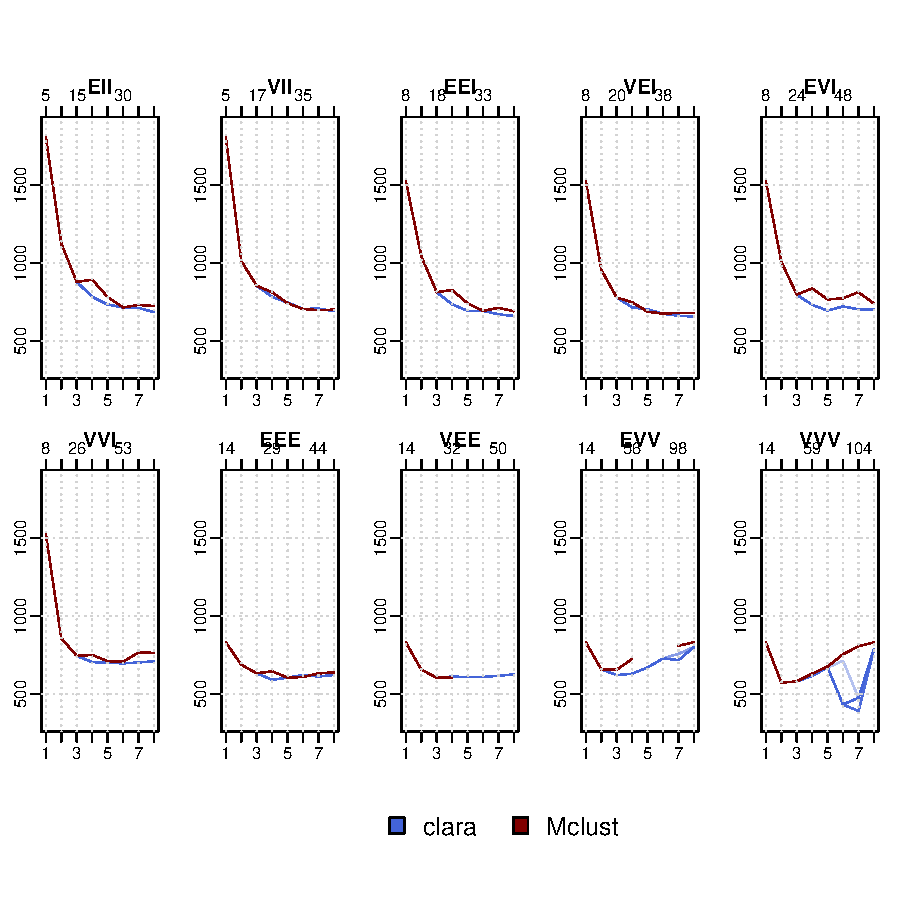
\includegraphics{chapter3-figtriris}
    \caption{The BIC values of the {\tt iris} data}
    \label{fig:triris}
    \end{Rgraph}
\end{figure}

The iris data originates from three types of plant species, which is not 
correctly identified by either {\tt norMmix} or {\tt mclust}. The best models
chosen are:

\begin{Schunk}
\begin{Soutput}
     model   count
[1,] "6 VVV" "18" 
[2,] "7 VVV" "7"  
\end{Soutput}
\end{Schunk}

Both far from three components. Furthermore {\tt mclust} does not return values
for some combinations of {\tt k} and {\tt model}. It is not clear what causes 
this, as a call to {\tt Mclust} simply returns {\tt NULL}.

Lastly, the data {\tt loss}, from the {\tt copula} package \cite{cop18}. This 
data is described as "Indemnity payment and allocated loss adjustment expense 
from an insurance company." It consists of $1500$ observations with $4$ 
variables. The BIC values are shown in \ref{fig:loss}

\begin{figure}[h!]
    \begin{Rgraph}[0.9]
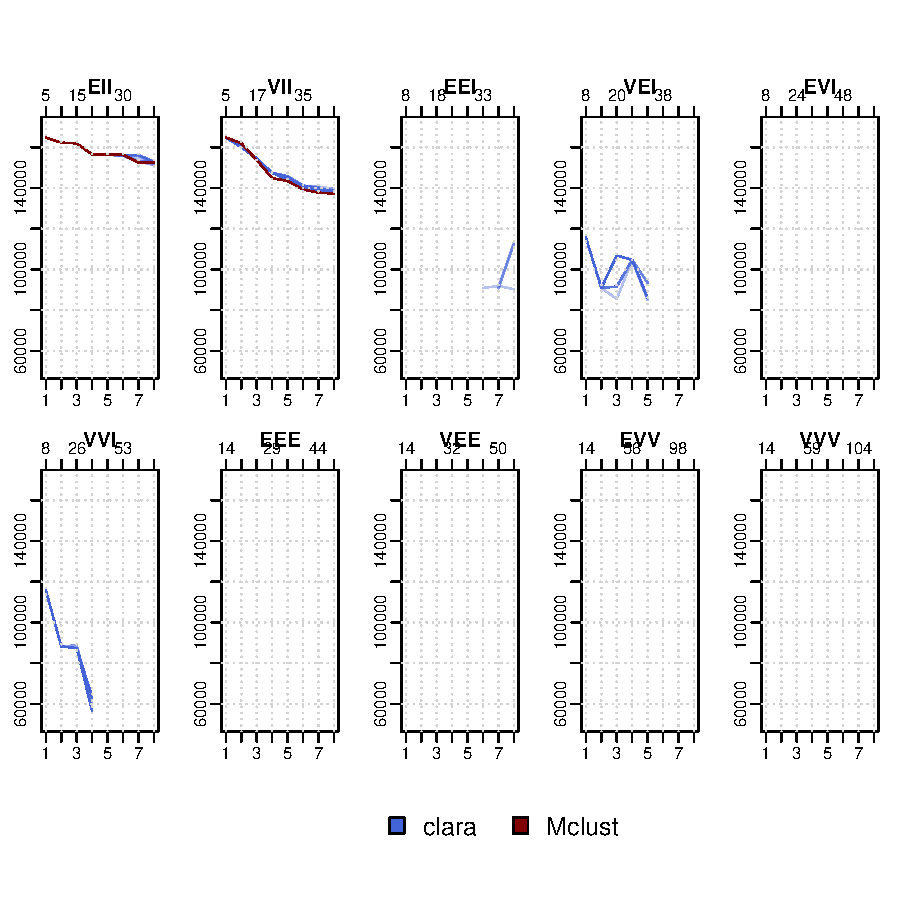
\includegraphics{chapter3-figloss}
    \caption{The BIC values of the {\tt loss}data}
    \label{fig:loss}
    \end{Rgraph}
\end{figure}

The data resists any attempt at fitting. {\tt mclust} returns {\tt NULL}, as 
with {\tt iris}. In {\tt norMmix}, the {\tt optim} function encounters an error.

\begin{Schunk}
\begin{Sinput}
>     data(loss, package="copula")
>     to <- try(norMmixMLE(loss, k=3, model="EEI"))
\end{Sinput}
\begin{Soutput}
initial  value 58082.835867 
iter  10 value 56418.201189
iter  20 value 53014.372756
iter  30 value 49490.970255
iter  40 value 46802.853871
\end{Soutput}
\begin{Sinput}
>     print(to)
\end{Sinput}
\begin{Soutput}
[1] "Error in optim(initpar., neglogl, method = method, control = control) : \n  non-finite finite-difference value [6]\n"
attr(,"class")
[1] "try-error"
attr(,"condition")
<simpleError in optim(initpar., neglogl, method = method, control = control): non-finite finite-difference value [6]>
\end{Soutput}
\end{Schunk}


\chapter{Discussion}



As we have seen, the algorithm works and is in many cases equal if not better 
to existing clustering methods. The approach is also very generalizable, with 
the biggest hurdle being an efficient implementation of a log-likelihood 
function and a parametrization strategy.
Should this approach be improved upon, it may provide a valuable tool in the
arsenal of mixture model analysis.

There are many directions further research in this area may be conducted. For 
instance, the initialization methods may prove to be an essential factor in 
correct model selection. Furthermore, in the case of CLARA, the parameters 
chosen are somewhat arbitrary. It could yield useful results how CLARA behaves 
with different sampling parameters.

The investigation conducted in this thesis also falls short in the study of 
high-dimensional datasets. While we have looked into it with the analysis of 
the {\tt SMI.12} data, the behaviour in these cases might also hold its own
difficulties, that have not cropped up in the study of one dataset.

Further research could also go in the direction of model selection theory. The 
Bayesian Information Criterion was chosen in this work for its reliable results
and usefulness, but other methods might yield more appropriate results.

There are also implementation related improvements, that could prove useful.
For example, as seen in figure \ref{fig:MW214bestfit}, spurious clusters are 
not accounted for at all in our implementation, which could strongly impact the
strength of this tool. This is most likely the most pressing issue with the 
implementation in this package, that no measures against spurious clusters
have been developed.


\section{Acknowledgements}

The Author would like to thank the 'Seminar f\"ur Statistik' and ETH Zurich 
for providing the computing resources needed for the simulations used in this
thesis. 

%% and more
% \include{....}
 
%%%%%%%%%%%%%%%%%%%%%%%%%%%%%%%%%%%%%%%%%%%%%%%%%
%%% Bibliography                              %%%
%%%%%%%%%%%%%%%%%%%%%%%%%%%%%%%%%%%%%%%%%%%%%%%%%
\addtocontents{toc}{\vspace{.5\baselineskip}}
% \cleardoublepage
\phantomsection
\addcontentsline{toc}{chapter}{\protect\numberline{}{Bibliography}}

\nocite{sfs19}
\nocite{mvt19}
\nocite{clu19}
\nocite{mix09}
\nocite{mas02}


\bibliography{References}
%% All books from our library (SfS) are already in a BiBTeX file
%% 'Assbib.bib' (included here as well), using
% \bibliography{myReferences,Assbib}
% ---------------------------------- instead of the above

%%%%%%%%%%%%%%%%%%%%%%%%%%%%%%%%%%%%%%%%%%%%%%%%% 
%%% Appendices (if needed, e.g. for R code)   %%%
%%%%%%%%%%%%%%%%%%%%%%%%%%%%%%%%%%%%%%%%%%%%%%%%%
\addtocontents{toc}{\vspace{.5\baselineskip}}
\appendix
\chapter{\Rp Code}


\section{{\tt llnorMmix}}

\lstinputlisting[firstline=1, lastline=211]{/home/n/ethz/BA/norMmix/R/llnorMmix.R}

\clearpage
\section{Example Simulation Script}

\label{App:sims}

\lstinputlisting{/home/n/ethz/BA/Rscripts/2time/2time.R}

\chapter{Further Plots}


\begin{Schunk}
\begin{Sinput}
>     library(norMmix, lib.loc="~/ethz/BA/norMmix.Rcheck/")
>     mainsav <- normalizePath("~/ethz/BA/Rscripts/")
\end{Sinput}
\end{Schunk}

\section{Behaviour in $n$}
\label{app:ben}

Here are the further plots ommited in section \ref{sec:ben}.
First is a very difficult mixture, ommited because it is studied in greater 
detail in section \ref{sec:def}. Second is a very easy mixture, because all
fitting lines overlap, making meaningful analysis futile.

\subsection{{\tt MW214}}

\begin{Schunk}
\begin{Sinput}
>     MW214
\end{Sinput}
\begin{Soutput}
norMmix object: 
multivariate normal mixture model with the following attributes:
name: 		 #14 Smooth Comb 
 model: 		 VII 
 dimension:	 2 
 components:	 6 
weight of components 0.5 0.1 0.1 0.1 0.1 0.1 
\end{Soutput}
\end{Schunk}


\begin{figure}[h!]
    \centering
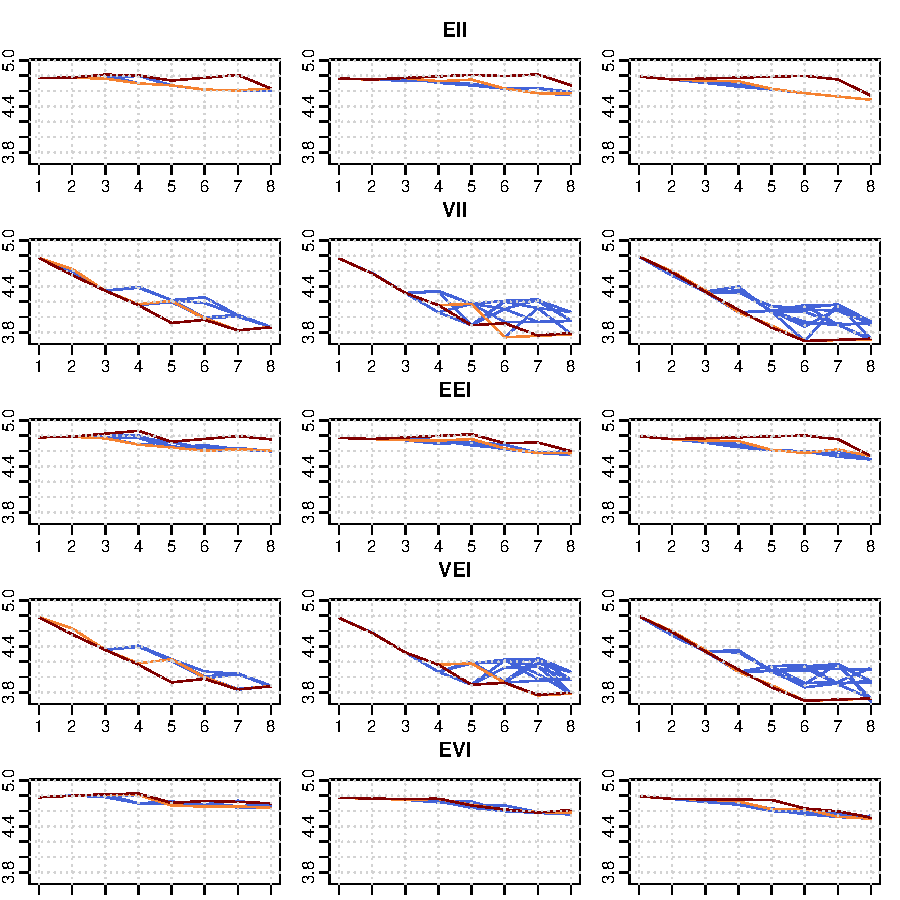
\includegraphics{App_plots-figmw21bicfirst}
    \caption{BIC values of {\tt MW214} with $n=\{500, 1000, 2000\}$, first five models}
    \label{fig:bicmw34first}
\end{figure}

\begin{figure}[h!]
    \centering
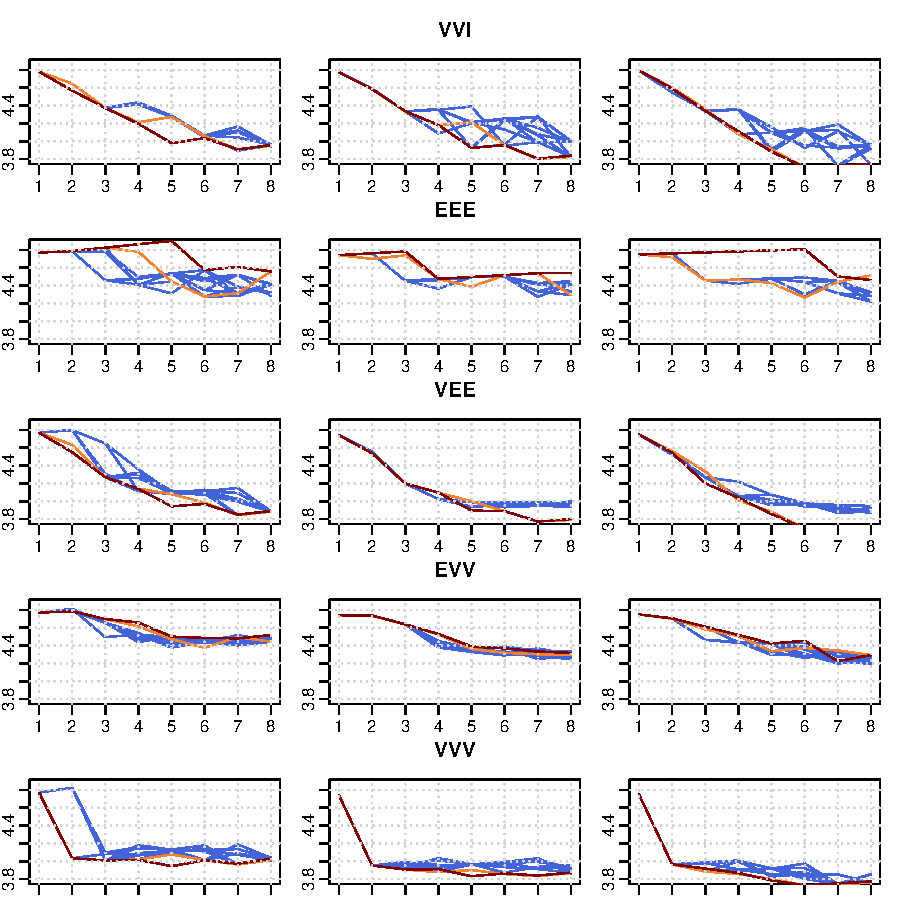
\includegraphics{App_plots-figmw21bicsecond}
    \caption{BIC values of {\tt MW214} with $n=\{500, 1000, 2000\}$, last five models.}
    \label{fig:bicmw34second}
\end{figure}

\clearpage

\subsection{{\tt MW51}}

\begin{figure}[h!]
    \centering
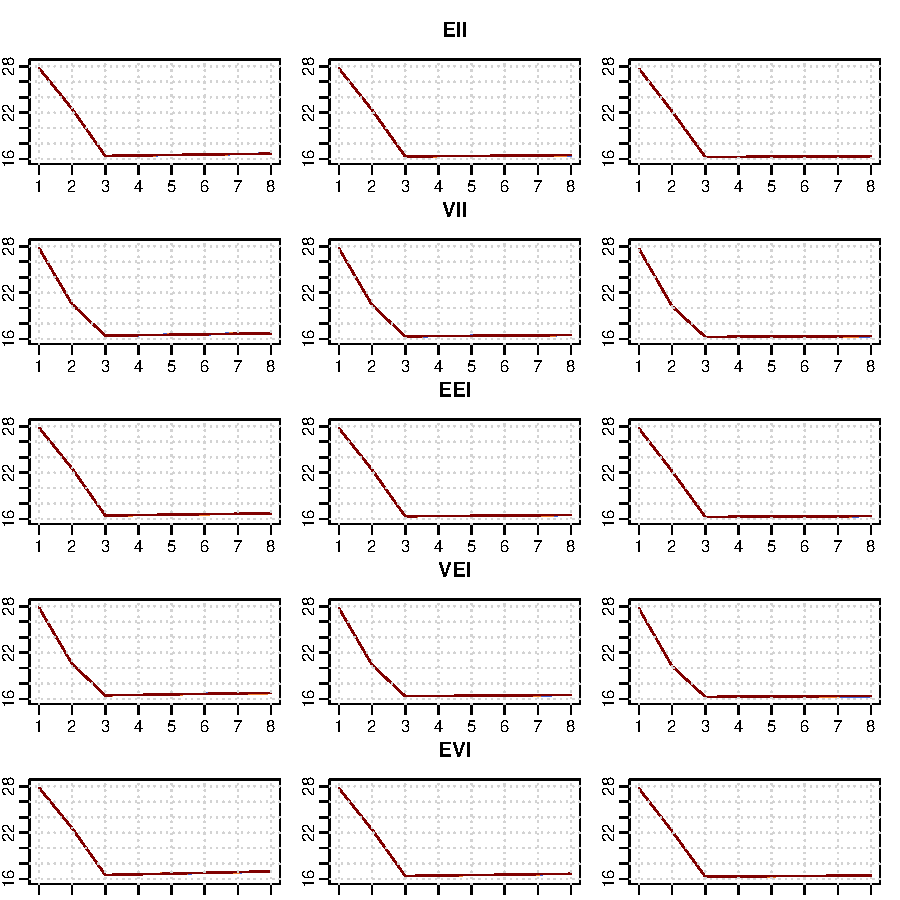
\includegraphics{App_plots-figmw51bicfirst}
    \caption{BIC values of {\tt MW51} with $n=\{500, 1000, 2000\}$}
    \label{fig:bicmw34first}
\end{figure}

\begin{figure}[h!]
    \centering
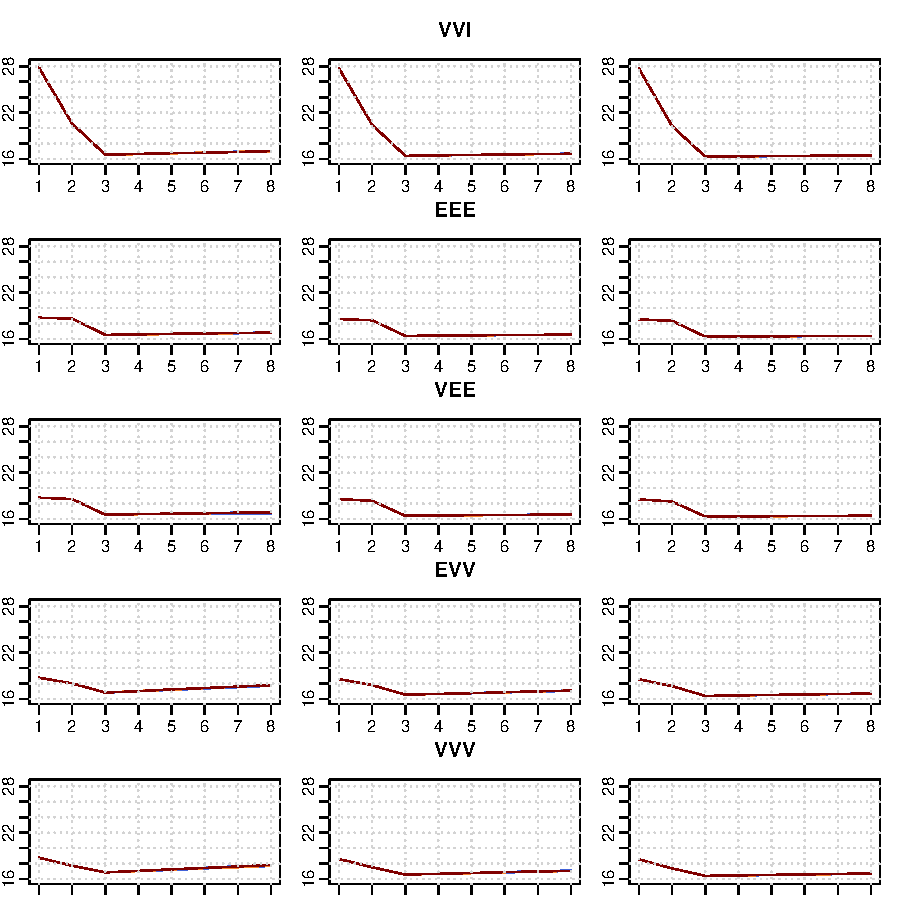
\includegraphics{App_plots-figmw51bicsecond}
    \caption{BIC values of {\tt MW51} with $n=\{500, 1000, 2000\}$}
    \label{fig:bicmw34second}
\end{figure}

\clearpage

\section{Other Data}

Unfortunately not all simulations were as useful to show in the main body of 
this work. In part, because they were done for exploratory purposes. However,
they show some other properties that are of interest.

The data in {\tt /simulations/smallinit} varied the dataset with a set seed.
The values for every individual dataset are not as interesting as 
{\tt /simulations/2time}, but they show that {\tt norMmix} is consistent in its
results for similar datasets.


\begin{figure}
    \centering
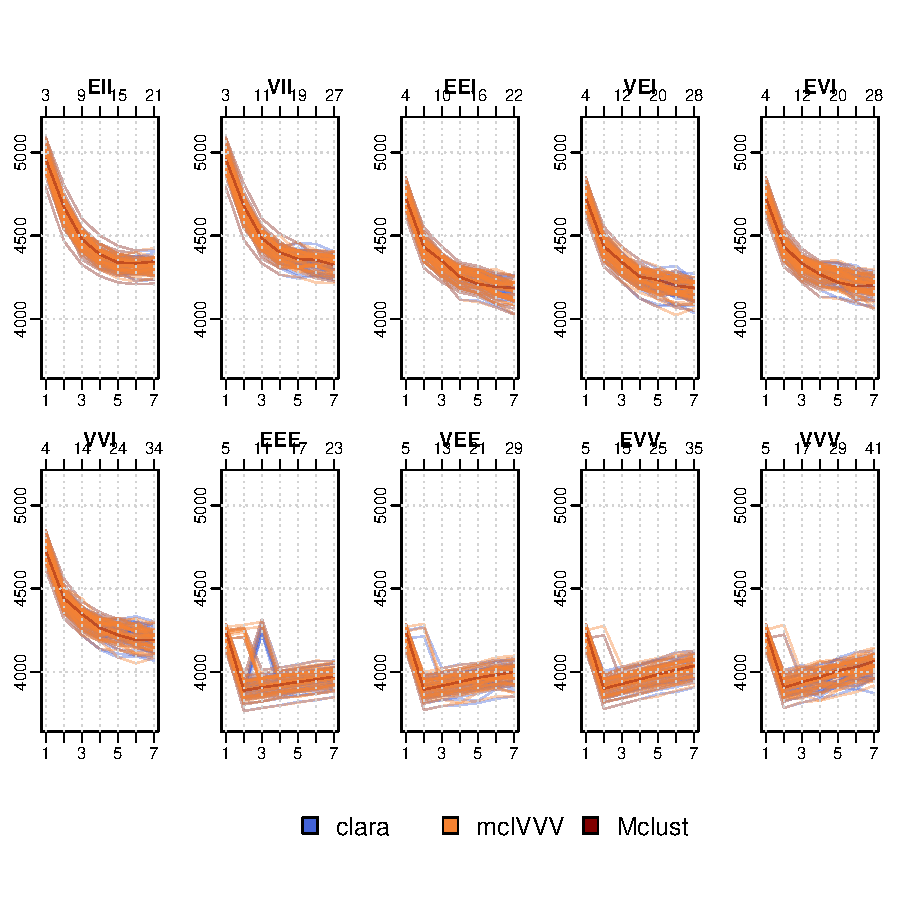
\includegraphics{App_plots-009}
\end{figure}

\begin{figure}
    \centering
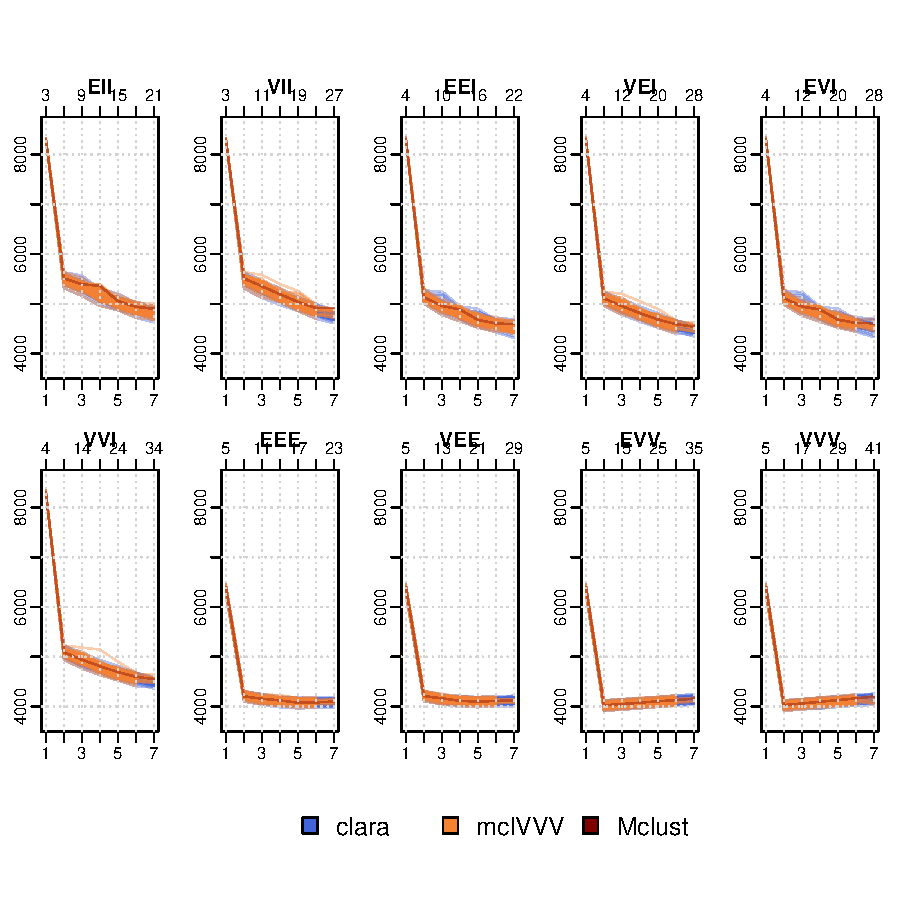
\includegraphics{App_plots-010}
\end{figure}

\begin{figure}
    \centering
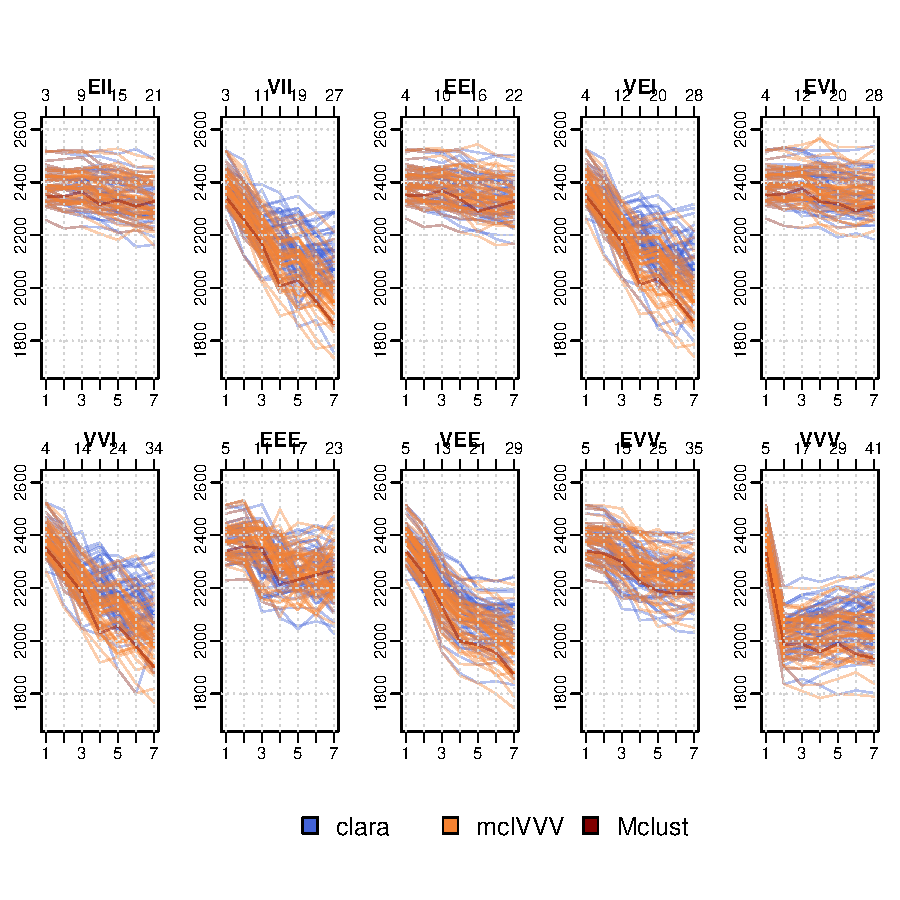
\includegraphics{App_plots-011}
\end{figure}

\begin{figure}
    \centering
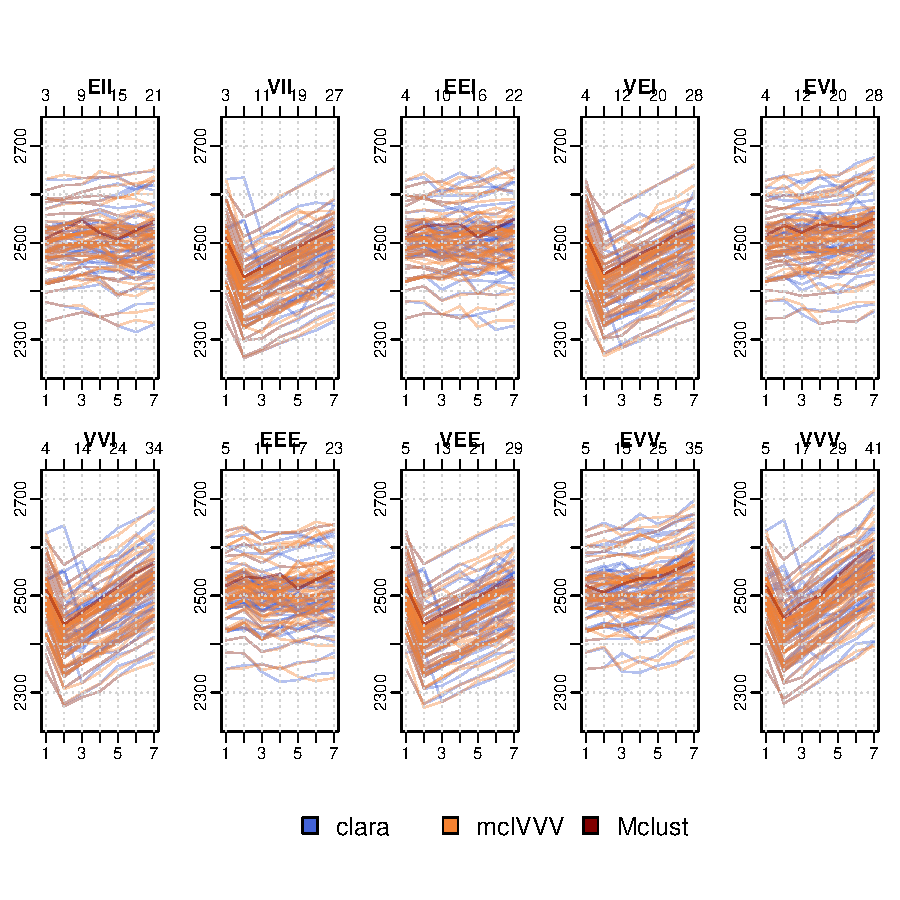
\includegraphics{App_plots-012}
\end{figure}

\begin{figure}
    \centering
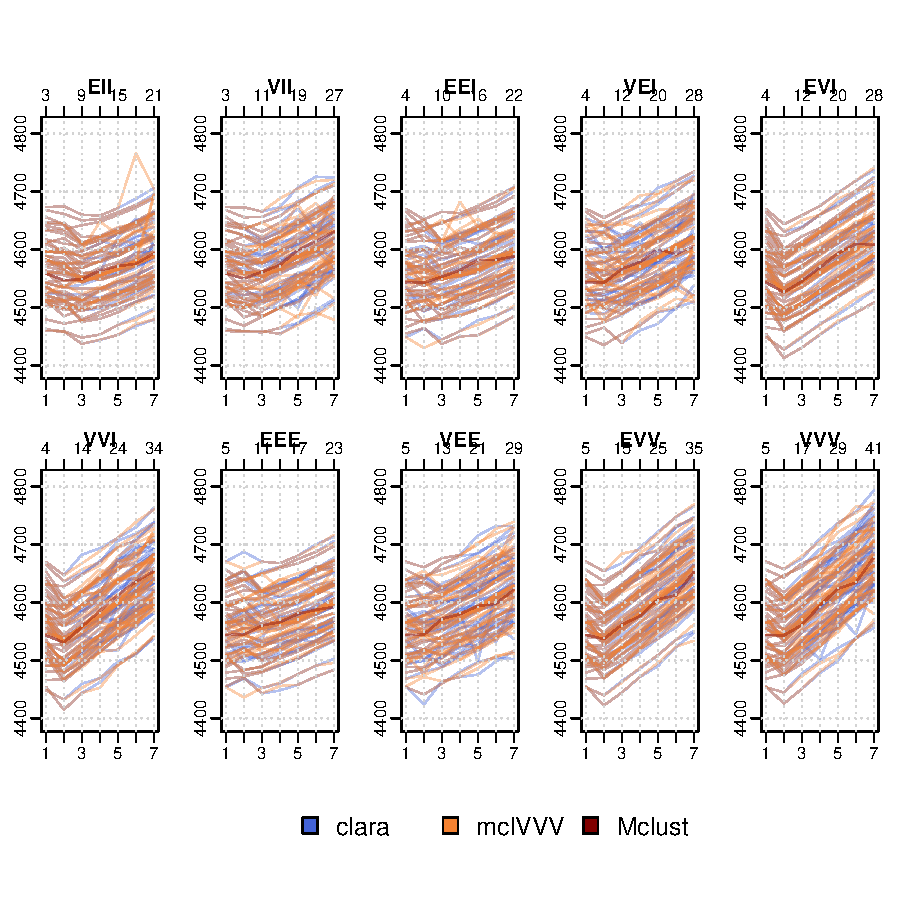
\includegraphics{App_plots-013}
\end{figure}

\begin{figure}
    \centering
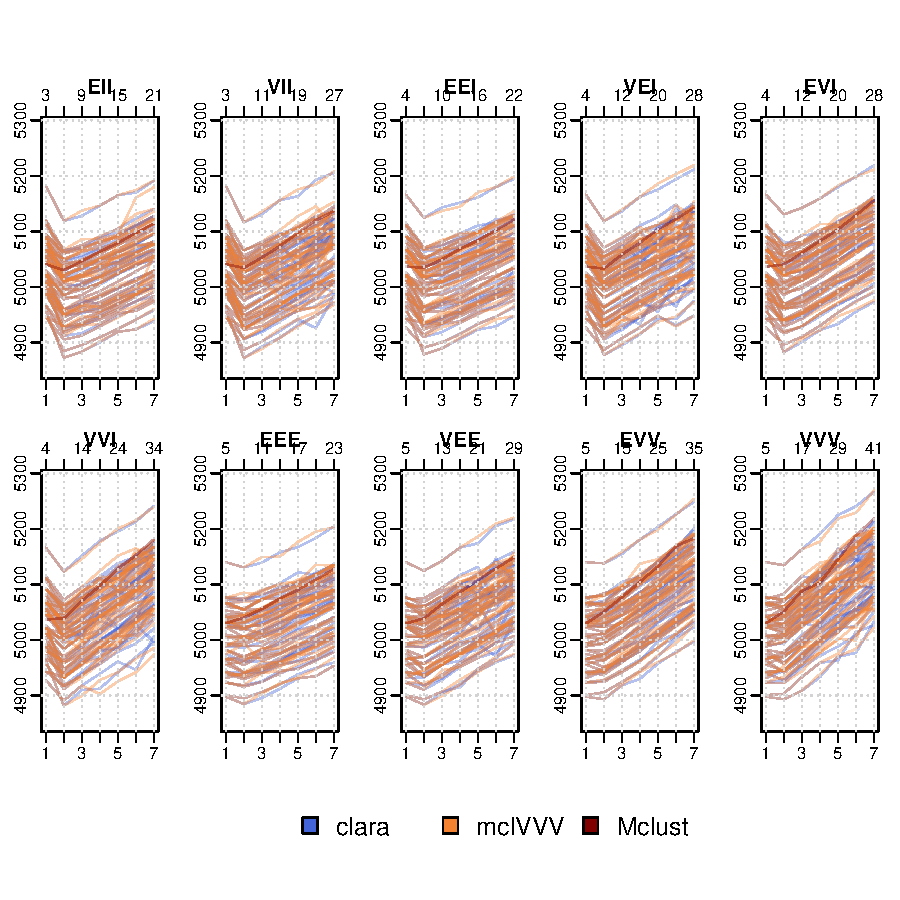
\includegraphics{App_plots-014}
\end{figure}

% outcommented \include{Appendix1}
% outcommented \include{Appendix_more_R}

%%%%%%%%%%%%%%%%%%%%%%%%%%%%%%%%%%%%%%%%%%%%%%%%%% 
%%% Declaration of originality (Do not remove!)%%%
%%%%%%%%%%%%%%%%%%%%%%%%%%%%%%%%%%%%%%%%%%%%%%%%%%
%% Instructions:
%% -------------
%% fill in the empty document confirmation-originality.pdf electronically
%% print it out and sign it
%% scan it in again and save the scan in this directory with name
%% confirmation-originality-scan.pdf 
%%
%% General info on plagiarism:
%% https://www.ethz.ch/students/en/studies/performance-assessments/plagiarism.html 
\cleardoublepage
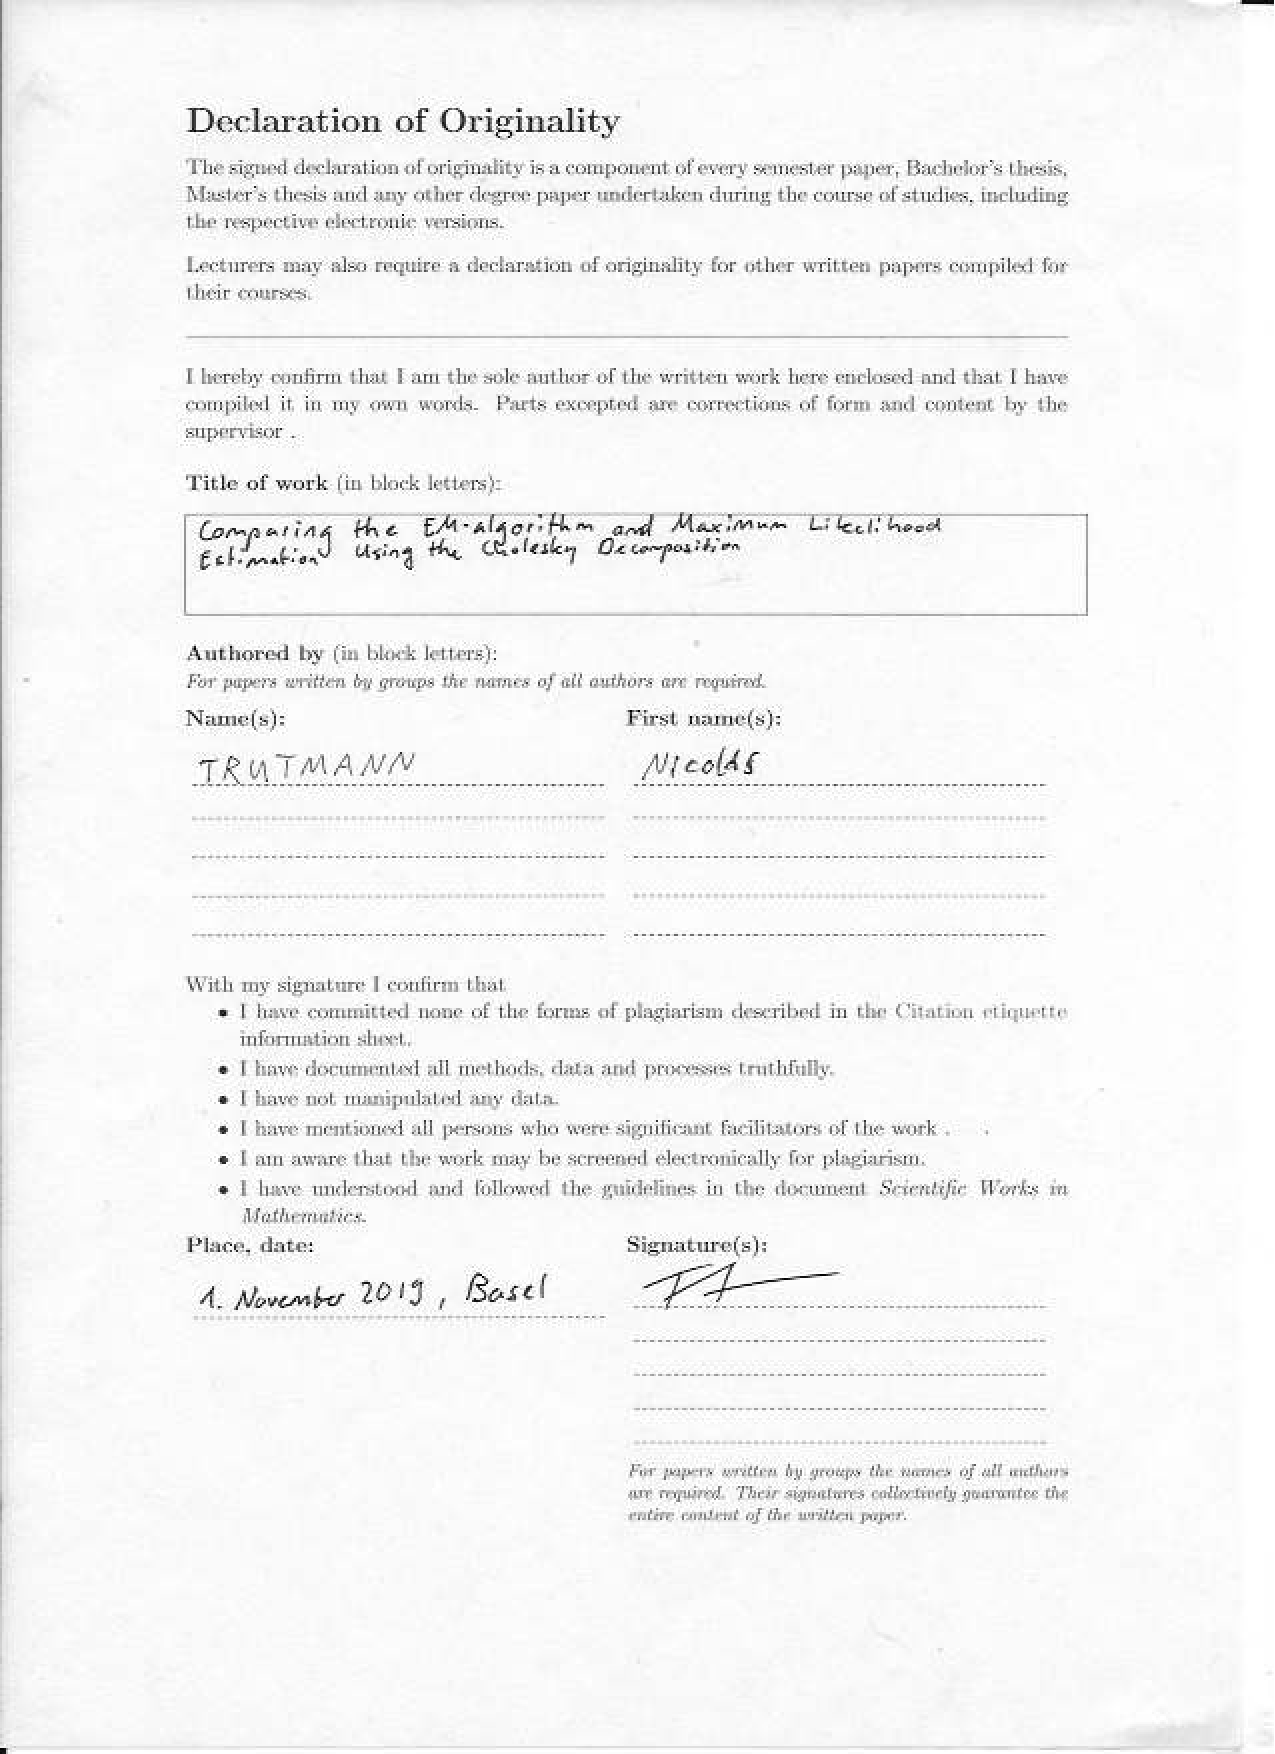
\includepdf[pages={-}, frame=true,scale=1]{DeclofOrig.pdf}
\end{document}
